
\documentclass[english,version-2020-11]{uzl-thesis}

% Copy this file as a template for your thesis. You will have to take
% action at all places marked by
%
% !!!!!!!!!!!!!!!!!!!!!!!!!!!!!!!!!!
% !!! Your action is needed here !!!
% !!!!!!!!!!!!!!!!!!!!!!!!!!!!!!!!!!
%
% The first place your action is needed is the first line of this
% document:
%
%
% Language of the thesis:
%
% You must use either 'german' or 'english' above, depending on the
% language used in the main text. This will automatically setup a lot
% of things in the background.
%
%
% Version of the class:
%
% You must specify which version of the thesis class is to be
% used. This is important in case the class style changes in later
% years, but we still want an older thesis to look the same, even when
% things are changed in the class.
%
% Do not change or remove the version-xxxx key.
%
%
% Text encoding:
%
% Your thesis *must* be encoded in utf8 (unicode), which is the
% default in most editors these days. Do *not* change this to latin8.



%%%
%
% Main setup:
%
%%%
%
% You must use the \UzLThesisSetup command to specify numerous things
% about your thesis. This includes the entries on the title page, the 
% abstracts, and the bibliography style. You do so by specifying
% so-called "values" for so-called "keys". For instance, 
% for the key "Autor" you must provide your name as the value. You do
% so by writing 'Autor = {Max Mustermann}', that is, the value is put
% into curly braces. You can use the \UzLThesisSetup command
% repeatedly and the order in which you provide the keys is not
% important. 
%
% Everything shown on the title page must be in German -- even
% if the thesis is written in English! Just insert German text for
% German keys and English text for English keys (like 'Abstract' needs
% English text, while 'Zusammenfassung' needs German text).

\UzLThesisSetup{
  %
  % !!!!!!!!!!!!!!!!!!!!!!!!!!!!!!!!!!
  % !!! Your action is needed here !!!
  % !!!!!!!!!!!!!!!!!!!!!!!!!!!!!!!!!!
  %
  % First, specify the institut or clinic at which the thesis was
  % written. You get the logo file from them (make sure it has the
  % correct size, namely the same as the example). If they do not have
  % a logo, the university's default logo is used.
  %
  % The 'verfasst' gets two arguments. Change the first to {an der}
  % for clinics, as in 'Verfasst = {an der}{Medizinischen Klinik I}'
  %
  Logo-Dateiname        = {logos/uzl-thesis-logo-itcs.pdf},
  Verfasst              = {am}{Institut für Theoretische Informatik},
  %
  % The titles:
  %
  Titel auf Deutsch     = {
    Vorlage für die \LaTeX-Klasse »uzl-thesis« zur Nutzung bei
    Bachelor-~und Masterarbeiten an der  Universität~zu~Lübeck
  }, 
  Titel auf Englisch    = {
    Template for the \LaTeX\ Class “uzl-thesis” for
    Bachelor's and Master's Theses Written at the University~of~Lübeck 
  },
  %
  % Author and supervisor:
  % 
  % Note that the 'Betreuer' or 'Betreuerin' is the supervisor, that
  % is, the professor who officially supervises the thesis. If there
  % is also an assistent of the professor who helped (typically a
  % lot), use 'Mit Unterstützung von' to thank that person. If the
  % thesis was mainly written 'externally' at some company or another
  % institute, point this out using 'Weitere Unterstützung'. 
  % 
  % For your own name, do *not* add things like "BSc" or "BSc
  % cand.". For the supervisor, you should normally include
  % "Prof. Dr." or "PD Dr." (ask your supervisor, what is
  % appropriate), but nothing more (so no
  % "Univ.-Prof. Dr. Dr. h.c. mult." unless your supervisor insists).  
  %
  Autor                 = {Max Mustermann (alias Till Tantau)},
  Betreuerin            = {Prof. Dr. Petra Wichtig-Wichtig},
  % 
  % Optional: Supporting persons and institutions. The text should be
  % in German, even for an English thesis.
  %
  Mit Unterstützung von = {Harry Hilfreich},
  % 
  %   Weitere Unterstützung = {
  %     Die Arbeit ist im Rahmen einer Tätigkeit bei der Firma Muster GmbH
  %     entstanden.
  %   },
  %
  %
  % Your Degree Programm (Studiengang)
  %
  % Specify 'Bachelorarbeit' or 'Masterarbeit' and the degree
  % programme. Make sure the name of programme is correct and not
  % some abbreviation or some incorrect variant. For instance:
  % 'Medizinische Ingenierwissenschaft', but not 'MIW';
  % 'Medizinische Informatik', but not 'Medizin-Informatik';
  % 'Informatik', but not 'Informatik (SSE)'.
  %
  % Use German names for German programmes and English names for
  % English ones, so 'Infection Biology', not 'Infektionsbiologie'. 
  % For programmes that have a German bachelor and an English master,
  % use the German name for a bachelor thesis and the English name for
  % the master thesis.
  %
  Bachelorarbeit,
  Studiengang           = {Informatik},
  %
  % Date on which the thesis is turned in German, formatted the
  % traditional German way:
  %
  Datum                 = {1. Januar 2021},
  %
  % The English abstract. You must always provide abstracts in German
  % and in English. 
  %
  Abstract              = {
    It is not easy to write a thesis that does not only advance
    science, but that is also a pleasure to read. While the scientific
    contribution of a thesis is undoubtedly of greater importance, the
    impact of \emph{writing well} should not be underestimated: If
    the person who grades a thesis finds no pleasure in the reading,
    that person are also unlikely to find pleasure in giving outstanding
    grades. A well-written text uses good German or English phrasing with a clear and correct 
    sentence structure and language rhythm, there are no spelling
    mistakes and the author's arguments are presented in a
    clear, logical and understandable manner using well-chosen
    examples and explanations. In addition, a nice-to-read font and a
    pleasing layout are also helpful. The \LaTeX\ class presented in
    this document helps with the latter: It contains a number of
    ready-to-use designs and 
    takes care of many small typographical chores.
  },
  Zusammenfassung       = {
    Es ist nicht leicht, eine Abschlussarbeit so zu schreiben, dass sie
    nicht nur inhaltlich gut ist, sondern es auch eine Freude ist, sie
    zu lesen. Diese Freude ist aber wichtig: Wenn die Person, die die 
    Arbeit benoten soll, wenig Gefallen am Lesen der Arbeit findet,
    so wird sie auch wenig Gefallen an einer guten Note
    finden. Glücklicherweise gibt es einige Kniffe, gut lesbare
    Arbeiten zu schreiben. Am wichtigsten ist zweifelsohne, dass
    die Arbeit in gutem Deutsch oder Englisch verfasst wurde mit klarem
    Satzbau und gutem Sprachrhythmus, dass keine Rechtschreib- oder
    Grammatikfehlern im Text auftauchen und dass die Argumente der
    Autorin oder des Autors klar, logisch, verständlich und gut
    veranschaulicht dargestellt werden. Daneben sind aber auch gut
    lesbare Schriftbilder und ein angenehmes Layout hilfreich. Die Nutzung
    dieser \LaTeX-Vorlage hilft der Schreiberin oder dem Schreiber
    dabei zumindest bei Letzterem: Sie umfasst gute, sofort nutzbare
    Designs und sie kümmert sich um viele typographische
    Details.  
  },
  %
  % Optional: 'Danksagungen' (German) or 'Acknowledgements'
  % (English). Both keys are optional and both have the same effect of
  % adding an acknowledgements text after the abstracts and before the
  % table of contents.
  %
  Acknowledgements      = {
    This is the place where you can thank people and institutions, do
    not try to do this on the title page. The only exception is in
    case you wrote your thesis while working or staying at a company or abroad. Then you
    should use the \Latex{Weitere Unterstützung} key to provide a text
    (in German) that acknowledges the company or foreign
    institute. For instance, you could use texts like »Die Arbeit
      ist im Rahmen einer Tätigkeit bei der Firma Muster GmbH
      entstanden« or »Die Arbeit ist im Rahmen eines
      Forschungsaufenthalts beim Institut für Dieses und Jenes an der
      Universität Entenhausen entstanden«. Do not name and thank
      individual persons from the company or foreign institute on the
      title page, do that here. 
  },
  % Bibliography style: Choose between
  % 
  % 'Alphabetische Bibliographie'
  % for all degree programmes in the natural sciences 
  % 
  % 'Numerische Bibliographie'
  % alternative for all other degree programmes
  % 
  % Either will load biblatex and setup the citation methods and the
  % bibliography styles correctly. You should not mess with them.
  % 
  %Alphabetische Bibliographie,
  % Alternatively:
  Numerische Bibliographie
}




%%%%%%%%%%%%%%%%%%%%
%
% Styling the thesis
%
%%%%%%%%%%%%%%%%%%%%
%
% Creating a visually pleasing layout and choosing fonts is not
% easy. Furthermore, different people have different preferences. Of
% course, for the University of Lübeck, the dean of studies could just
% force everyone to use one specific layout and font, but that seems a
% bit drastic and, also, it seems nice that thesis by different people
% have an individual style even though they all stick to the same
% overall structure.
%
% For these reasons, I (Till Tantau) have spend quite some time on
% designing a flexible layout and styling mechanism for theses.
%
% Basically, the overall structure of the thesis is fixed by the
% thesis class and so are many structural elements. For instance, you
% cannot change the order in which the abstract and table of contents
% are shown, you cannot move the bibliography elsewhere, indeed, the
% bibliography style is also fixed. Likewise, the text on the title
% page is fixed.
%
% Although many things are fixed, you *can* change several other
% things. For instance, you can change the font used for the main
% text, you can change which font is used for titles and headings or
% you can change whether titles and headlines are centered or flushed
% left.
%
% There are many LaTeX packages for changing such things. You are
% kindly asked *not to use them*. Rather, use (only) the options
% offered by the thesis class. All possible choices and combinations
% there have been tested by me and produce nice results; what happens
% with other packages no one knows and might no longer conform to what
% is expected by the university. As you will see, you still have a
% lot of options.
%
%
% Technical note: All styling is done via the command
%
% \UzLStyle{...}
%
% where ... is a key-value list just as for \UzLThesisSetup. The
% difference is just that everything having to do with styling as
% controlled by \UzLStyle, while the more “formal” setup keys are
% controlled by \UzLThesisSetup.
%
%%%
%
% Designs
%
%
% A \emph{design} is a whole set of font and layout options bundled
% together. They have been chosen in such a way that a visually
% pleasing “overall appearance” results.
%
%
% \UzLStyle{computer modern oldschool design}
%
% The look of this design mimics the “classical” way a paper or report
% created with \LaTeX\ looks like: The Computer Modern font is used,
% bold face fonts are used for headlines, only black and white are
% used as colors. This design reminds me of older scientific
% documents, especially from the computer science community where
% \LaTeX\ was used very early.
%
%
% \UzLStyle{computer modern basic design}
%
% A slightly less “oldschool” version of the previous design. It is
% still a classic design in the sense that it uses the Computer Modern
% font and that it still has this “good old \LaTeX” look, but some
% more modern aspects (like colors!) have been added.
%
% Note that this design uses Myriad for the title page (one of the
% “modern aspect”), which means that his font must be installed.
%
%
% \UzLStyle{computer modern scholary design}
%
% In my opinion, this is the ultimate “scholary design”: The thesis
% will look like it has been typeset by hand some 150 years ago and
% then printed by a university press. There is really nothing “modern”
% about it and the word in the name of the design is just part of the
% name of the “Computer Modern” font.
%
%
% \UzLStyle{pagella basic design}
%
% A, well, basic design that uses the Pagella font rather than the
% Computer Modern font. Especially the bold face version of this font
% looks nicer than the Computer Modern counterpart. Also, Pagella,
% while still having a “bookish” look, still feels a bit fresher than
% Computer Modern. 
%
%
% \UzLStyle{pagella centered design}
%
% A variant of the basic Pagella design that centers all
% headlines. A nice alternative to the basic version.
%
%
% \UzLStyle{pagella contrast design}
%
% This design tries to create some visual friction by contrasting the
% sans serif headline font (in bold!) with the main text. I find it a
% visually very interesting combination.
%
%
% \UzLStyle{alegrya basic design}
%
% The third variant of the basic design, this time using the Alegrya
% font. 
%
%
% \UzLStyle{alegrya scholary design}
%
% The Alegrya version of the previous “scholary” design. Unlike the
% Computer Modern version, this design does not look old, but more
% fresh -- while still creating the impression that the text must be
% about a very scientific subject. 
%
%
% \UzLStyle{alegrya stylish design}
%
% The design is quite similar to the scholary version for the Alegrya
% font, but with even more modern additions. “Stylish” is the word
% that comes to my mind.
%
%
\UzLStyle{alegrya modern design}
%
% A design that uses the sans serif version of the Alegrya font for
% the headlines. This is a nice modern overall design.
%
%%%




%%%%%%%%
%
% Now, include the package you need here using \usepackage. 
%
% However, many standard packages are already loaded by the class:
%
% amsmath, amssymb, amsthm, babel, biblatex, csquotes, etoolbox,
% filecontents, fontspec, geometry, hyperref, tikz (with libraries
% arrows.meta, positioning and shapes), varioref, url 
%
% Indeed, in many cases you will not need any extra packages.
%
%%%%%%%
\usepackage{cleveref}
\usepackage{multirow}
\usepackage{subcaption}

\begin{document}

%
% The title page and table of contents will be inserted automatically
% here. 
%

\chapter{Introduction}
% In a German thesis write: \chapter{Einleitung}


The increasing complexity of modern automotive systems has led to a growing
demand for precise in-cabin monitoring technologies. Among these, 
steering wheel detection plays a pivotal role in monitoring driver
behavior, enhancing safety, and facilitating autonomous control in 
advanced driver-assistance systems. Estimating the 3D location and 
orientation of the steering wheel is crucial for systems that rely on
driver interaction and vehicle control. 
Yet, achieving accurate 3D detection of such an object within a car's 
interior presents unique challenges, including variations in rotation and
position within confined, occlusion-prone environments. This is because 
the car's interior is a complex and constrained environment, with limited 
sensor coverage and frequent occlusions of key components like the 
steering wheel. Accurately determining the 3D position and orientation of 
the steering wheel is essential for enabling advanced driver monitoring 
and assistive technologies, but poses significant technical hurdles 
compared to object detection in open, outdoor environments. 


\section{Contributions of This Thesis}
This thesis addresses the problem of steering wheel detection using 3D 
point cloud, which offers a rich representation of spatial information. 
Specifically, this research contributes in two significant ways: 

First, it introduces a novel dataset that represents the car interior, 
including 3D point clouds and annotated bounding boxes for the steering 
wheel. This dataset was created through a meticulous process involving 
the recording of point cloud data, feature extraction, and preprocessing 
to ensure data integrity and clarity. By accurately determining the 
steering wheel’s 3D position and orientation, this dataset serves as a 
critical foundation for model training and validation.

Second, this thesis proposes a model-based approach for detecting the 
steering wheel’s 3D position using a modified VoxelRCNN architecture. 
Existing 3D object detection models, such as those trained on KITTI 
dataset data, are typically optimized for outdoor environments with 
non-cubic point cloud dimensions and restricted rotational degrees of 
freedom (DOF). To overcome these limitations, the research modifies the VoxelRCNN 
architecture to account for a cubic point cloud structure and allows for rotation detection along 
the x-axis, which is crucial for accurately representing the orientation of the steering wheel.

\section{Structure of This Thesis}
This thesis is organized to guide the reader through the development of a dataset and model for 3D steering wheel detection within the context of in-cabin monitoring for autonomous driving. Chapter 1, \textbf{Introduction}, presents the motivation for this research and highlights the specific contributions of this thesis. Chapter 2, \textbf{Related Work}, provides an overview of the existing literature on 3D object detection in autonomous driving, covering detection methods, commonly used datasets, and performance metrics, along with a summary of current challenges in the field.

Chapter 3, \textbf{Creating Dataset}, details the process of building a custom dataset for steering wheel detection. This includes data collection, preprocessing, ground truth generation, and the experiments conducted to validate the dataset. Both an initial and refined approach to ground truth generation are discussed, with results presented to evaluate the dataset’s effectiveness. Chapter 4, \textbf{Estimating Steering Wheel Position}, focuses on the architecture and adaptations made to a 3D object detection network for accurately detecting the steering wheel. It includes an evaluation of the model’s performance based on the developed dataset. The thesis concludes with Chapter 5, \textbf{Conclusion}, summarizing the key findings and suggesting directions for future research.




\chapter{Background and related works}
In this section, we explore the foundational concepts and advancements 
in 3D object detection techniques that are relevant to 
in-cabin monitoring and steering wheel detection. Given the critical 
role of perception in autonomous driving, achieving robust and reliable 
3D detection of interior components like the steering wheel has become a 
key challenge in this field. This chapter presents an overview of 
various 3D object detection methods, focusing on point cloud-based 
approaches, multimodal fusion techniques, and image-based approaches. 
We also discuss the unique challenges posed by interior environments, 
including issues such as occlusions, irregular lighting conditions, 
and limited rotational freedom for 3D bounding boxes, which make 
existing detection methods difficult to apply directly to car interior 
scenarios. Finally, we provide an overview of publicly available 
datasets and the key performance metrics commonly used in 3D object 
detection for autonomous driving, assessing their relevance and 
applicability for interior monitoring applications.


\section{3D Object Detection in Autonomous Driving}
3D object detection in autonomous driving enables the vehicle to
understand and perceive its surrounding environment by identifying, 
localizing, and characterizing nearby objects. In this context, 
3D detection provides both precise spatial positioning and orientation 
information for objects, making it an essential component for crucial 
tasks such as path planning, collision avoidance, and motion prediction.
However, current 3D object detection methods are primarily optimized 
for exterior, outdoor environments, where sensor setups, object dynamics, 
and available datasets differ significantly from the more constrained and
complex interior scenarios found within a vehicle. Outdoor 3D detection
has greatly benefited from the availability of large-scale datasets like 
KITTI, nuScenes, and Waymo, which provide extensive labeling for objects 
in open, relatively unobstructed spaces, captured under varied lighting 
and weather conditions. These datasets and approaches, however, 
do not adequately address the intricacies and unique challenges 
involved in detecting objects within a vehicle's constrained and 
complex interior space.

\subsection{Challenges in 3D Detection for Interior Monitoring}
Detecting objects in the car interior, specifically the steering wheel, 
involves overcoming several challenges:
\begin{itemize}
    \item \uzlemph{Limited Field of View (FOV)}: Unlike outdoor detection, 
    where sensors cover a 360° view around the vehicle, interior sensors 
    are constrained to the car’s internal structure, resulting in 
    limited and often obstructed views of certain objects.
    \item \uzlemph{Occlusions and Sparse Data}: Objects like the steering
    wheel may be partially or fully occluded by the driver’s hands or 
    other interior elements, and point cloud data from LiDAR or other 
    depth sensors can be sparse due to occlusion and reflective surfaces.
    \item \uzlemph{Variability in Rotational Degrees of Freedom (DOF)}: While 
    outdoor models assume limited rotational DOF (often around the z-axis for vehicles), 
    steering wheel detection requires accurate modeling of rotation 
    around the x-axis to capturithe essential rotational characteristics 
    of the steering wheel.
    \item \uzlemph{Adaptability to Point Cloud Dimensions}: Standard point 
    clouds from datasets like KITTI have unbalanced dimensions, favoring 
    a broader lateral view. In contrast, interior point clouds are 
    typically cubic, and models must adapt to these differences for 
    effective detection.
\end{itemize}


\section{3D Object Detection Methods}
3D object detection techniques are generally categorized based on the 
input modality (image-based, point cloud-based, or multimodal fusion) 
and architecture type (two-stage, single-stage, or hybrid). 
\Cref{3d_object_detection_Categorization} shows a summary of the key approaches and their characteristics.

\begin{table}[htpb]
    \caption{Categorization of 3D object detection approaches by input modality and architecture type}
    \label{3d_object_detection_Categorization}
    \centering
    \begin{tabular}{|l r l|}
        \uzlhline
        \hspace{1cm} \uzlemph{Category} & \multicolumn{2}{c|}{\hspace{-1cm}\uzlemph{Method}} \\
        \uzlhline
        \uzlemph{Image-Based Methods} & \uzlemph{Result-Lifting} & Stereo R-CNN \cite{stereo_rcnn}\\
        & \uzlemph{Feature-Lifting} & Pseudo-LiDAR \cite{pseudo_lidar}\\
        &  & Pseudo-LiDAR++ \cite{pseudo_lidar++}\\
        &  & DSGN \cite{dsgn}\\
        & & \\
        \uzlemph{Point Cloud-Based Methods} & \uzlemph{Voxel-Based} & VoxelNet \cite{voxnet} \\
        &  & VoxelRCNN \cite{voxelrcnn} \\
        &  & SE-SSD \cite{se_ssd} \\
        &  & BtcDet \cite{bdc_det} \\
        
        & \uzlemph{Point-Based} & PointRCNN \cite{point_rcnn} \\
        &  & Point-GNN \cite{point_gnn}\\
        &  & PointNet++ \cite{pointnet++}\\
        & \uzlemph{Hybrid} & PV-RCNN \cite{pv_rcnn} \\
        & & \\
        \uzlemph{Multimodal Fusion-Based} & \uzlemph{Early Fusion} & AVOD \cite{avod} \\
        &  & MV3D \cite{mv3d} \\
        & \uzlemph{Deep Fusion} & PointPainting \cite{pointpainting} \\
        & \uzlemph{Sequential} & Frustum PointNets \cite{frustum_pointnet} \\
        \hline
    \end{tabular}
\end{table}
\subsection{Image-Based Methods}
Image-based 3D detection methods rely on RGB images or stereo images 
to infer depth and spatial information. These methods are cost-effective 
and widely applicable, but they lack direct depth information, 
which makes it challenging to accurately localize objects in 3D space. 
Image-based approaches typically involve:
\begin{itemize}
    \item \uzlemph{Result-Lifting}: Detecting objects in 2D and projecting 
    their bounding boxes to 3D space based on geometric constraints or 
    templates, as in methods like Stereo R-CNN \cite{stereo_rcnn}.
    \item \uzlemph{Feature-Lifting}: Estimating depth maps from images 
    and creating pseudo-LiDAR \cite{pseudo_lidar} point clouds, 
    which can then be processed similarly to actual LiDAR data. 
    Approaches like Pseudo-LiDAR++ \cite{pseudo_lidar++} and 
    DSGN \cite{dsgn} have shown promising results, but 
    they still struggle with accuracy over long distances and under 
    variable lighting, which is especially problematic in the dimly lit car interiors.
\end{itemize}


\subsection{Point Cloud-Based Methods}
Point cloud-based methods are better suited for direct 3D localization, 
using data from LiDAR or other depth sensors to create dense, spatial 
representations. These methods can be further divided into voxel-based, 
point-based, and hybrid approaches:
\begin{itemize}
    \item \uzlemph{Voxel-Based Methods}: VoxelNet \cite{voxnet} 
    and its successors, such as VoxelRCNN \cite{voxelrcnn}, 
    partition the point cloud into voxel grids and apply convolutional 
    operations, capturing spatial structure but at a high computational 
    cost. Another effective voxel-based approach is 
    SE-SSD (Self-Ensembling Single-Stage Detector) \cite{se_ssd} 
    that improves on voxel-based approaches by using a student-teacher 
    framework. The student model learns from a teacher model that is 
    refined with additional structure-aware information, improving 
    robustness and accuracy in challenging conditions such as occlusions 
    and sparse point clouds. Another voxel-based approach, 
    BtcDet \cite{bdc_det}, focuses on long-range and sparse 
    data detection. BtcDet enhances detection performance in challenging 
    scenes by using shape-adaptive learning to manage low-quality data, 
    which is particularly useful in adverse weather or complex scenes.
    \item \uzlemph{Point-Based Methods}: Approaches like 
    PointRCNN \cite{point_rcnn} and 
    Point-GNN \cite{point_gnn} use permutation-invariant 
    operations on raw point clouds, maintaining fine-grained details 
    but often requiring high computational resources and memory. 
    For example, PointNet++ \cite{pointnet++} , 
    a popular point-based method, hierarchically extracts features 
    from individual points, preserving fine-grained geometric details 
    but demanding significant computational power.
    \item \uzlemph{Hybrid Methods}: Combining voxel and point approaches, 
    methods like PV-RCNN \cite{pv_rcnn} aim to balance 
    computational efficiency with spatial accuracy by processing both 
    coarse-grained voxel features and fine-grained point details. 
    This hybrid approach has proven advantageous for complex environments but 
    has yet to be fully adapted for indoor environments with unique constraints, 
    like a car interior.
\end{itemize}


\subsection{Multimodal Fusion-Based Methods}
Multimodal fusion combines RGB images and point cloud data to enhance detection 
accuracy by leveraging complementary data. Early, deep, and late fusion 
strategies vary based on when the modalities are combined in the model. 
PointPainting \cite{pointpainting}, for example, demonstrates 
deep fusion by blending intermediate features from both modalities, 
while methods like AVOD \cite{avod} and 
MV3D \cite{mv3d} 
rely on early fusion to incorporate image information directly into the point 
cloud processing pipeline. 
Additionally, Frustum PointNets \cite{frustum_pointnet}, for instance, 
fuses LiDAR and image features within 3D frustums projected from 2D object 
detection results, effectively reducing the search space for 3D object detection. 
However, aligning features between images and point clouds in indoor 
environments poses significant challenges, particularly due to spatial 
and view misalignments.



\section{Datasets for 3D Object Detection in Autonomous Driving}
The field has developed multiple benchmark datasets, each with unique attributes 
for testing 3D detection models:
\begin{itemize}
    \item \uzlemph{KITTI}: One of the earliest and most influential datasets, 
    KITTI \cite{kitti} 
    includes over 200,000 labeled objects captured in outdoor urban settings. 
    However, its limited class diversity and lack of interior scenes make it 
    less suitable for in-cabin monitoring.
    \item \uzlemph{nuScenes} \cite{nuscenes}\uzlemph{ and Waymo} \cite{waymo}: 
    These datasets provide richer scenes, diverse weather and lighting 
    conditions, and multimodal data, including LiDAR, radar, and cameras. 
    Although they cover more object classes than KITTI, they still focus on 
    outdoor scenarios.
\end{itemize}
The absence of publicly available in-cabin datasets emphasizes the need 
for specialized datasets to meet the requirements of car interior 
monitoring tasks.


\section{Performance Metrics for 3D Object Detection}
3D object detection performance is commonly evaluated through metrics 
such as Average Precision (AP) and mean Average Precision (mAP).
Additional metrics include:
\begin{itemize}
    \item \uzlemph{Intersection over Union (IoU)}: 
    IoU evaluates the overlap between predicted and ground truth bounding 
    boxes. For autonomous driving, models are often tested at varying IoU 
    thresholds depending on object size and importance.
    \item \uzlemph{NuScenes Detection Score (NDS)} and \uzlemph{Average Precision with Heading (APH)}: 
    Used in the nuScenes and Waymo datasets, these metrics account for 
    orientation and other attributes specific to 3D space, offering a 
    comprehensive measure of performance for complex scenes.    
\end{itemize}


\section{Summary}
In summary, while 3D object detection has seen substantial advancements 
in outdoor environments, these methods face limitations when applied to 
in-cabin monitoring. The unique challenges of interior environments 
require adapted models, tailored datasets, and precise metrics that can 
account for both spatial constraints and occlusions. In the following 
chapters, we detail our approach to address these gaps by creating a 
dedicated dataset and adapting a 3D object detection model, optimized 
for steering wheel detection and localization within a confined interior 
space.

\chapter{SWD dataset}

The unique constraints of in-cabin monitoring and the specific 
requirements for steering wheel detection necessitated the development 
of a custom dataset. Existing datasets, such as KITTI and nuScenes, 
predominantly focus on external vehicle perception, capturing objects 
like cars, pedestrians, and road signs. These datasets are tailored 
for outdoor environments and often lack the spatial resolution, 
balance, and context required for confined in-cabin spaces. 
Furthermore, the irregular rotational degrees of freedom (DOF) in 
interior setups, along with occlusions and limited sensor viewpoints, 
further complicate the application of outdoor 3D detection models to 
in-cabin scenarios.

To address these limitations, a dataset specifically designed for 
steering wheel detection was developed, incorporating high-quality 3D 
point clouds and ground truth bounding boxes to capture the full 3DOF 
of the steering wheel’s position and 

The diversity in subjects, poses, and conditions in this dataset 
provides a comprehensive foundation for training and evaluating 3D 
object detection models specifically for steering wheel estimation. 
The following sections outline the methodology used for recording, 
data extraction, and ground truth generation, detailing the steps 
taken to produce high-fidelity 3D representations suitable for 
accurate steering wheel detection and orientation modeling.


\section{Recording Procedure}
To accurately capture the steering wheel's position across multiple 
configurations, I set up a recording protocol using a board with 
ArUco markers\footnote{\url{https://docs.opencv.org/3.4/db/da9/tutorial_aruco_board_detection.html}} 
centered on the steering wheel as shown in \cref{fig:demo_model}. 
ArUco board helps with estimating position and orientation of 
the steering wheel in 3D space.  A positional reference card, 
similar to \cref{fig:reference_board}, was placed adjacent to the steering wheel, displaying 
16 distinct steering wheel orientations for standardized positioning. 
This approach allowed me to systematically record the steering wheel 
in various orientations, providing a comprehensive dataset for training 
and evaluating 3D object detection models focused on steering wheel 
estimation.

The video recordings were conducted using an Azure Kinect camera 
embedded in a car demo model as demonstrated in \cref{fig:demo_model}. 
This camera was positioned on the ceiling, slightly over the driver’s 
shoulder, and angled to capture the entire steering wheel. 

\begin{figure}[ht]
    \centering
    \begin{subfigure}[t]{0.45\textwidth}
        \centering
        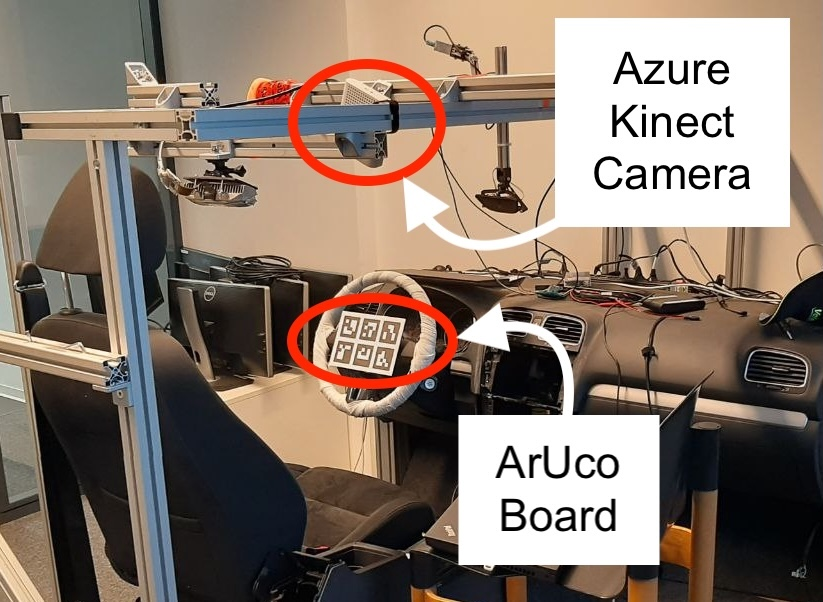
\includegraphics[width=\textwidth]{media/chapter 3/demo_model.jpg}
        \caption{ArUco board placed at the center of the steering wheel 
        and the Azure Kinect camera over the driver's shoulder 
        on the aluminium frames.}
        \label{fig:demo_model}
    \end{subfigure}\hfill
    \begin{subfigure}[t]{0.45\textwidth}
        \centering
        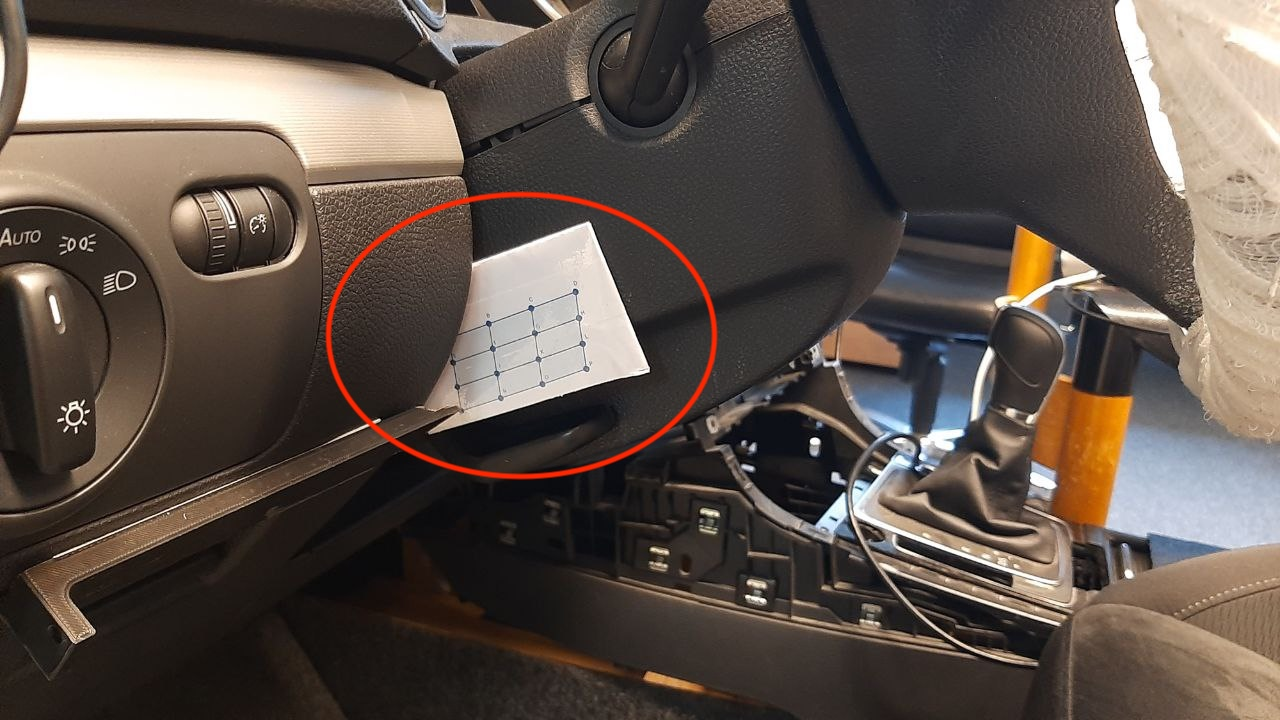
\includegraphics[width=\textwidth]{media/chapter 3/reference_board.jpg}
        \caption{A reference card was positioned next to the 
        steering wheel, illustrating 16 unique steering wheel orientations 
        to ensure standardized alignment.}
        \label{fig:reference_board}
    \end{subfigure}
    \caption{The demo model setup used for recording streams.}
\end{figure}

The dataset was composed of recordings from 10 unique participants, 
with each participant engaging with the steering wheel in 16 distinct 
orientations. To introduce variability, the participants wore various 
accessories during the recordings. 
This resulted in a comprehensive dataset encompassing 72,747 training 
frames, 42,712 validation frames, and 29,099 testing frames. 
The steering wheel itself was covered with a white fabric to 
reduce reflections and enhance detection accuracy.

The dataset was recorded in two phases for each subject. 
First, a ground truth stream was captured with no driver 
present and the marker board fully visible as shown in \cref{fig:gt_stream}. 
This short footage was used to extract accurate ground truth data on 
the position and orientation of the steering wheel. 
Subsequently, a second stream was recorded with the driver 
interacting with the steering wheel, simulating a driving 
scenario. During these main recordings, the marker board was 
covered with a black surface to prevent unintended biases in 
the model training as illustrated in \cref{fig:main_stream}. 
The driver performed typical driving 
actions, such as steering with one or both hands, operating 
the dashboard, and other natural behaviors. 

For data processing, ground truths were extracted from the initial 
ground truth streams, while the main streams with the driver were 
used to extract point clouds for further experimentation.

\begin{figure}[ht]
    \centering
    \begin{subfigure}[t]{0.45\textwidth}
        \centering
        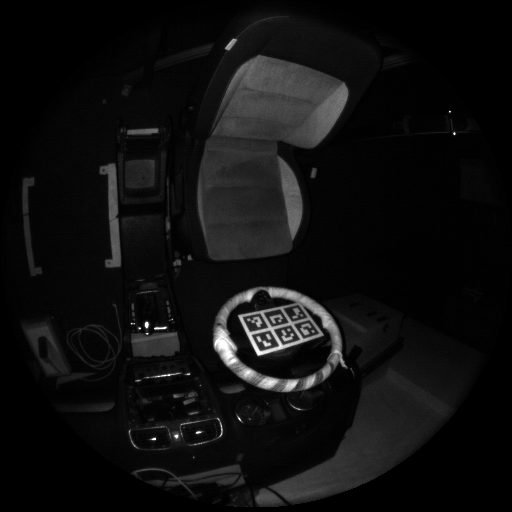
\includegraphics[width=\textwidth]{media/chapter 3/gt_stream.png}
        \caption{Ground truth data on the steering wheel’s 
        position and orientation were obtained from a stream 
        recorded without a driver, ensuring full visibility 
        of the marker board.}
        \label{fig:gt_stream}
    \end{subfigure}\hfill
    \begin{subfigure}[t]{0.45\textwidth}
        \centering
        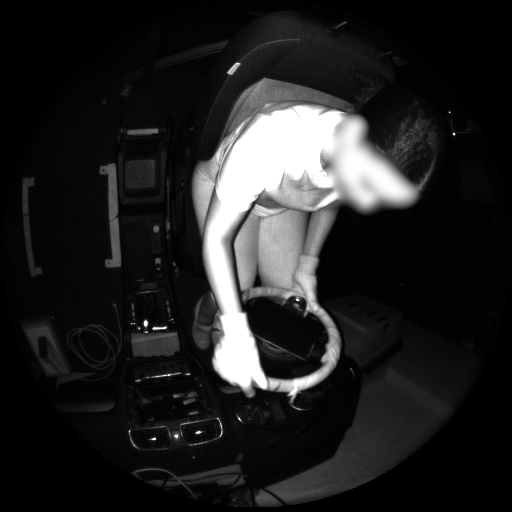
\includegraphics[width=\textwidth]{media/chapter 3/main_stream.png}
        \caption{A second stream was recorded with the driver 
        interacting with the steering wheel, simulating a 
        driving scenario, while the marker board was covered 
        to prevent biases in model training.}
        \label{fig:main_stream}
    \end{subfigure}
    \caption{Two stages of recording streams.}
\end{figure}

\section{Data Extraction}
In the initial data extraction phase, depth and amplitude 
information was derived from the video streams to create 
high-quality point clouds. The raw point clouds were then refined 
through a series of preprocessing steps to enhance their quality 
and suitability for accurate steering wheel position detection:

\begin{itemize}
    \item \textbf{Noise Reduction}: Filtering out extraneous points to 
    achieve a clear and uncluttered point cloud.
    \item \textbf{Distortion Correction}: Applied using 
    OpenCV's distortion matrices to enhance the clarity and accuracy 
    of both depth and amplitude images.
    \item \textbf{Edge Removal}: Points on the edges of the point cloud 
    were omitted due to their ambiguous positioning, which could 
    reduce the overall accuracy of the model.
    \item \textbf{Cropping}: The point cloud was cropped to a 
    50cm x 50cm x 50cm area around the steering wheel, ensuring that 
    the data was focused and relevant for model training and reducing 
    the dataset size.
\end{itemize}

These comprehensive preprocessing steps helped to create precise, 
refined point clouds that were well-suited for accurately detecting 
the position of the steering wheel.


\section{Ground Truth}
To generate ground truth data for the steering wheel's position and 
orientation, I explored two approaches due to the challenges presented 
by point sparsity and data distortion. The first approach, which 
involved annotating 2D points on images of the steering wheel and then 
mapping them to 3D space, failed to accurately represent the true 
position and orientation of the steering wheel. This was because the 
sparse and noisy distribution of the sampled points resulted in an 
imprecise oriented bounding box that did not capture the steering 
wheel's actual location and orientation with sufficient precision. 

In contrast, the second approach using ArUco markers \cite{opencv_aruco_detection} 
and plane fitting proved to be a much more effective method. 
By first accurately estimating the 3D location of the ArUco markers and then fitting a 
plane to the markers' board, I was able to precisely determine the 
steering wheel's location and orientation with three degrees of freedom. 
This method overcame the limitations of the initial approach and 
provided high-quality ground truth data that could be used for 
training and evaluating 3D object detection models.

Each approach will be discussed in more detail in the following sections.

In this dataset, the ground truth for each frame includes an 
oriented bounding box that represents the precise 3D position 
and orientation of the steering wheel. Bounding boxes are 
encoded as \([x, y, z, l, w, h, rx, ry, rz]\), 
where \((x, y, z)\) represents the center of the bounding box, 
\((l, w, h)\) represents the dimensions of the box, 
\((rx, ry, rz)\) represent the bounding box angle with 
the \(x\), \(y\), and \(z\) axes, respectively. 
\Cref{fig:sample_obbs} illustrates the ground truth data and oriented 
bounding boxes for sample frames from the dataset, 
providing a comprehensive visual representation of the 
steering wheel's 3D position and orientation.

\begin{figure}[ht]
    \centering
    \begin{subfigure}[t]{0.3\textwidth}
        \centering
        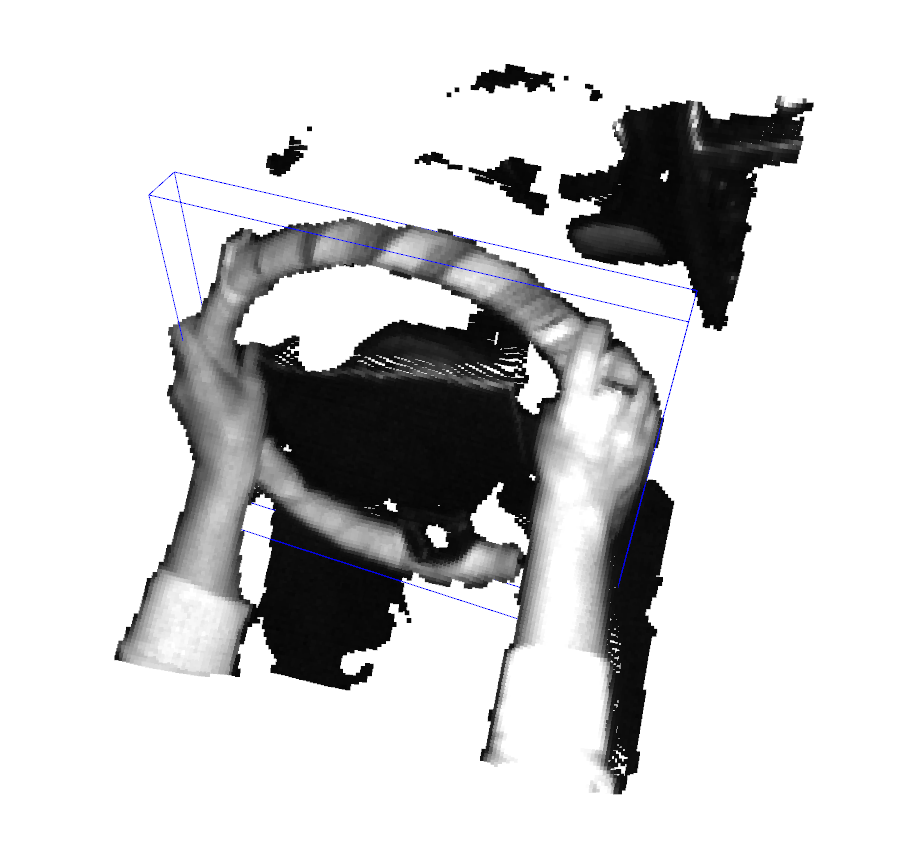
\includegraphics[width=\textwidth]{media/chapter 3/obb1.png}
    \end{subfigure}\hfill
    \begin{subfigure}[t]{0.3\textwidth}
        \centering
        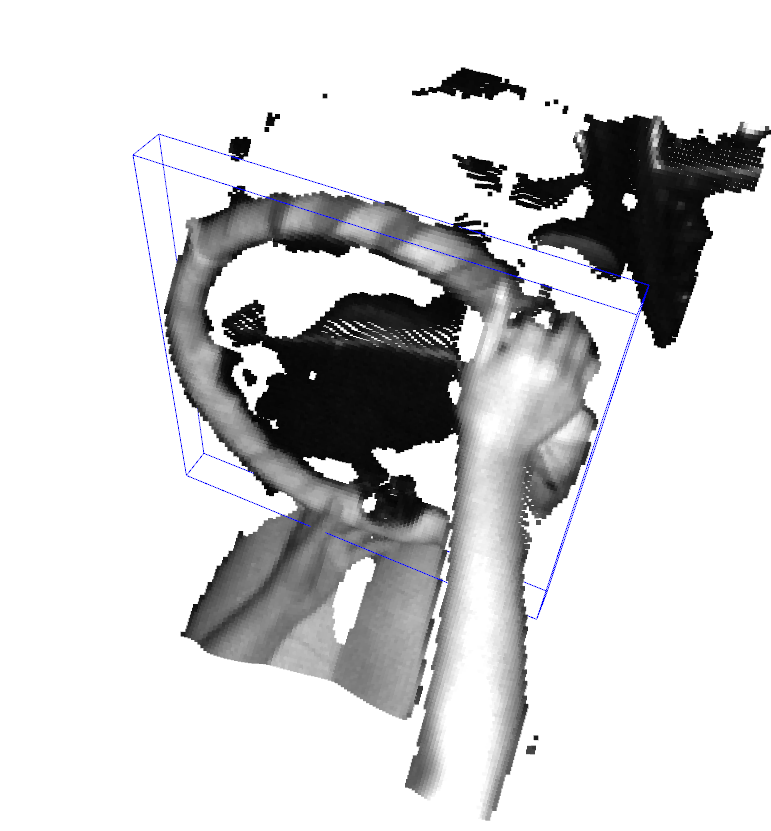
\includegraphics[width=\textwidth]{media/chapter 3/obb2.png}
    \end{subfigure}\hfill
    \begin{subfigure}[t]{0.3\textwidth}
        \centering
        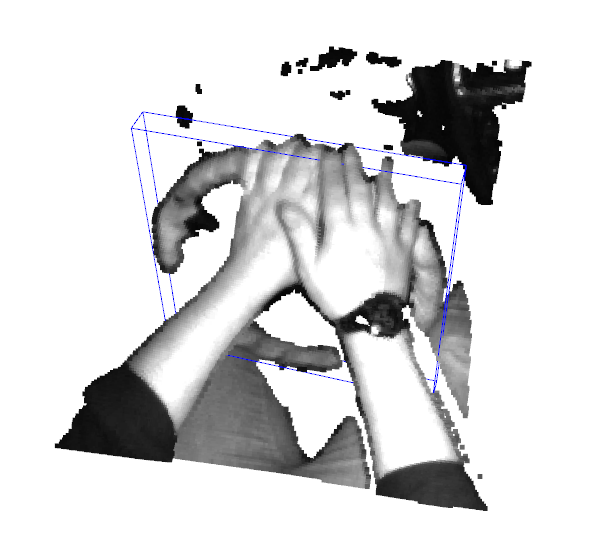
\includegraphics[width=\textwidth]{media/chapter 3/obb3.png}
    \end{subfigure}\\
    \begin{subfigure}[t]{0.3\textwidth}
        \centering
        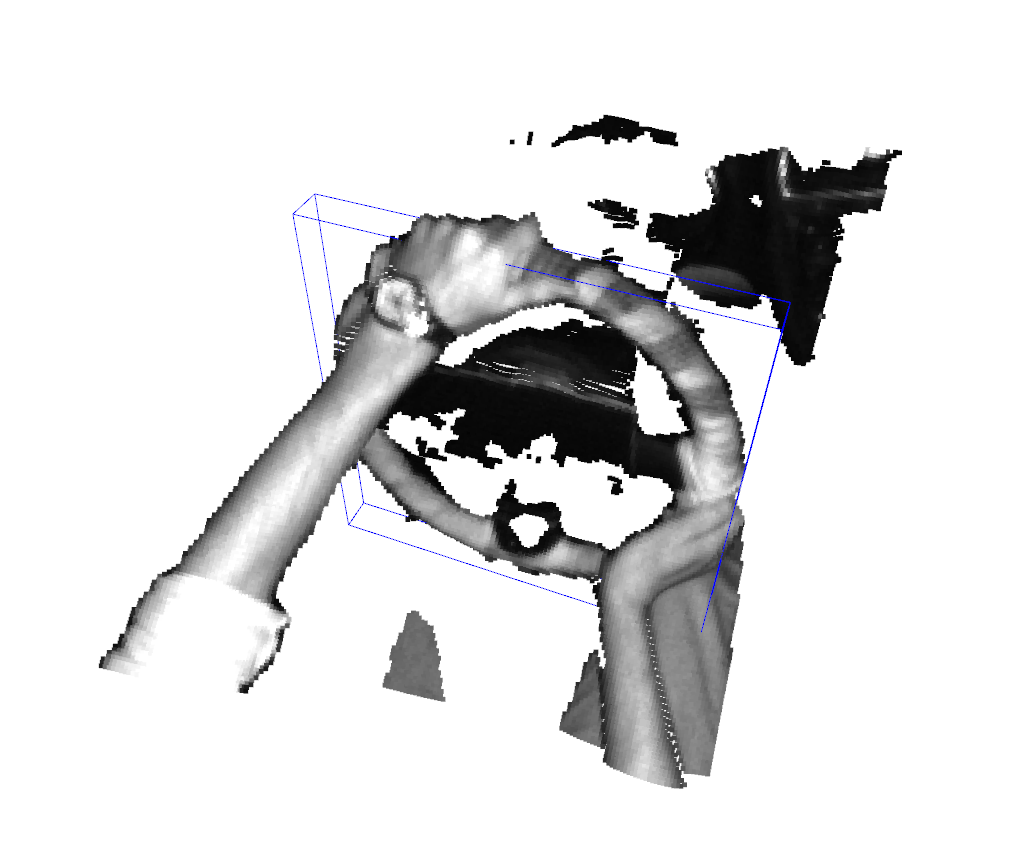
\includegraphics[width=\textwidth]{media/chapter 3/obb4.png}
    \end{subfigure}\hfill
    \begin{subfigure}[t]{0.3\textwidth}
        \centering
        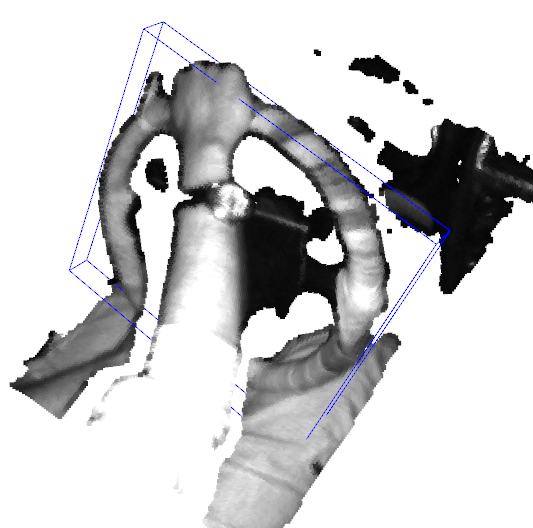
\includegraphics[width=\textwidth]{media/chapter 3/obb5.png}
    \end{subfigure}\hfill
    \begin{subfigure}[t]{0.3\textwidth}
        \centering
        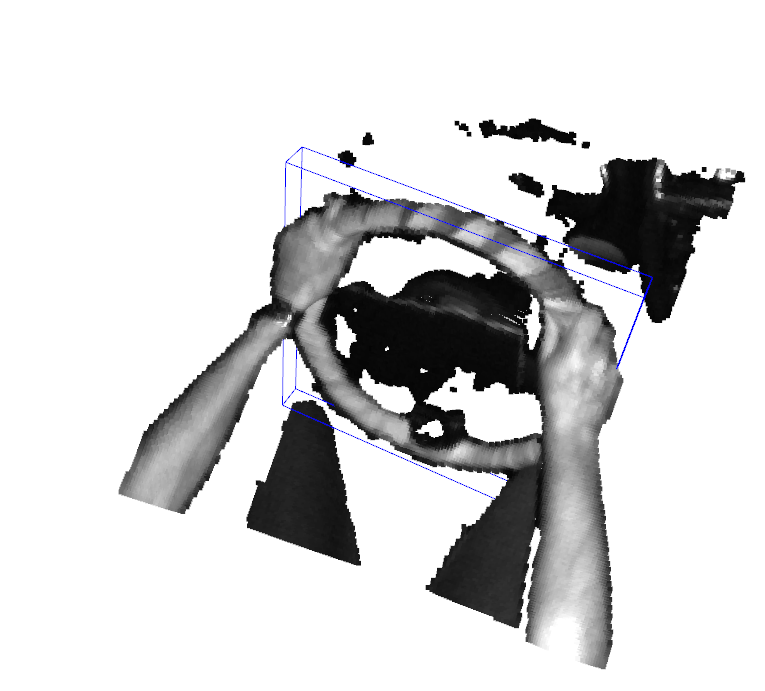
\includegraphics[width=\textwidth]{media/chapter 3/obb6.png}
    \end{subfigure}
    \caption{oriented bounding boxes for sample frames from the dataset}
    \label{fig:sample_obbs}
\end{figure}


Given the ground truths, we can also represent the steering wheel 
as a torus shape, as depicted in \cref{fig:sample_toruses}. 
The torus shape can provide a more accurate geometric 
representation of the steering wheel, capturing its circular 
cross-section and three-dimensional nature more effectively 
than a bounding box. By modeling the steering wheel as a 
torus, we can better account for its curvature and overall 
shape, which is essential for accurate 3D pose estimation and 
object detection tasks.


\begin{figure}[ht]
    \centering
    \begin{subfigure}[t]{0.3\textwidth}
        \centering
        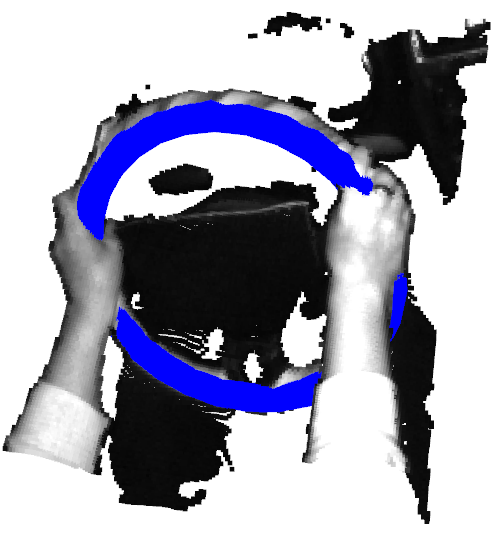
\includegraphics[width=\textwidth]{media/chapter 3/torus1.png}
    \end{subfigure}\hfill
    \begin{subfigure}[t]{0.3\textwidth}
        \centering
        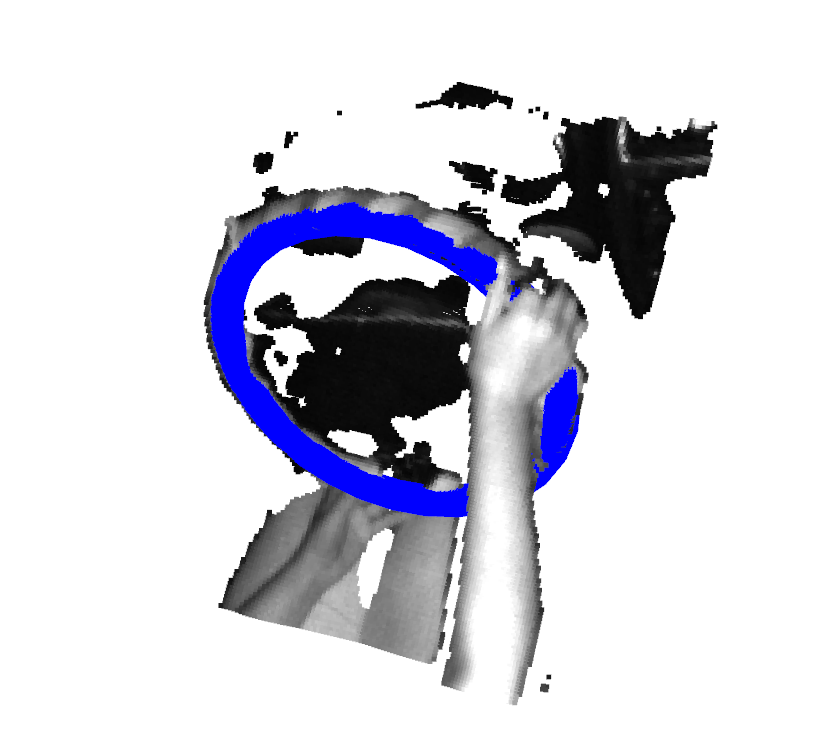
\includegraphics[width=\textwidth]{media/chapter 3/torus2.png}
    \end{subfigure}\hfill
    \begin{subfigure}[t]{0.3\textwidth}
        \centering
        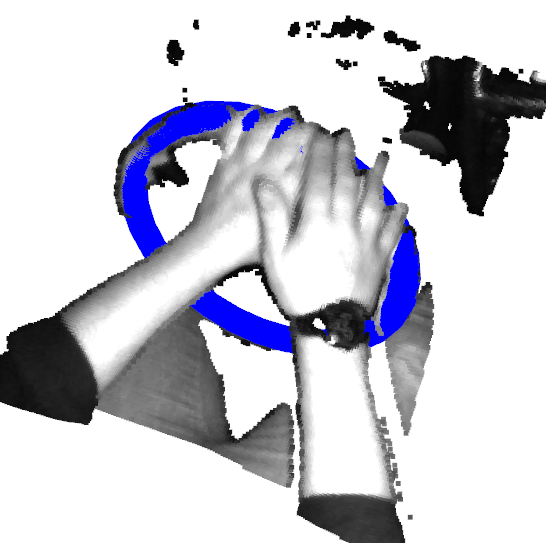
\includegraphics[width=\textwidth]{media/chapter 3/torus3.png}
    \end{subfigure}\\
    \begin{subfigure}[t]{0.3\textwidth}
        \centering
        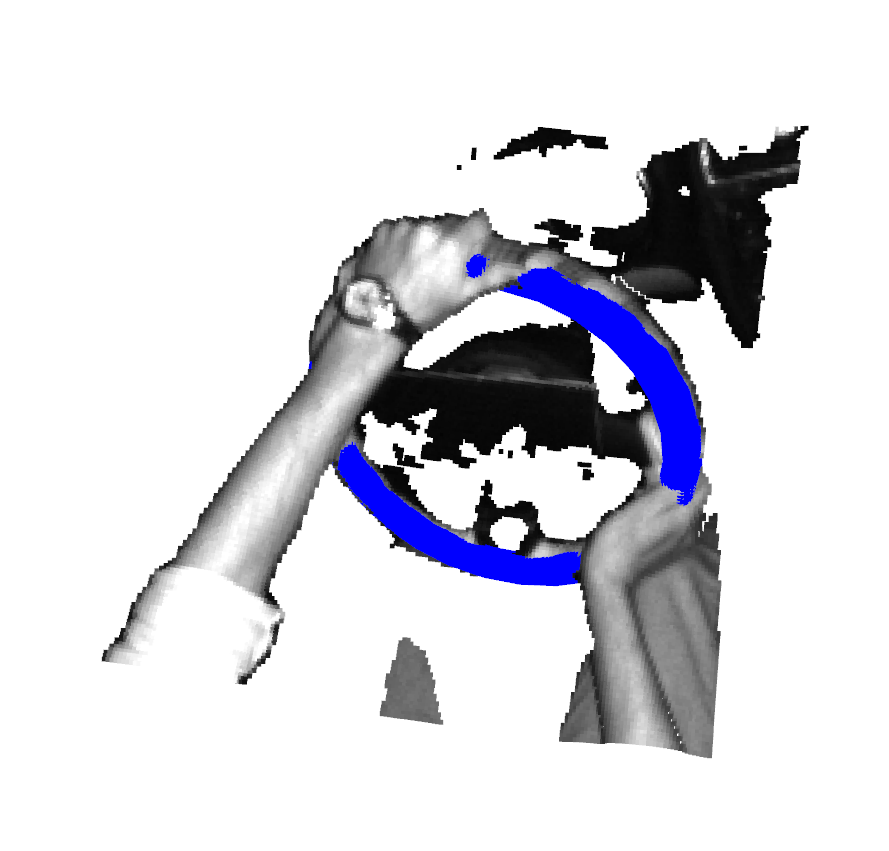
\includegraphics[width=\textwidth]{media/chapter 3/torus4.png}
    \end{subfigure}\hfill
    \begin{subfigure}[t]{0.3\textwidth}
        \centering
        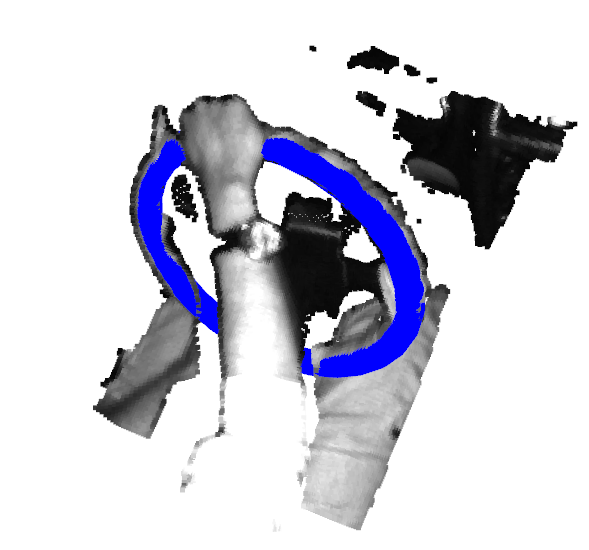
\includegraphics[width=\textwidth]{media/chapter 3/torus5.png}
    \end{subfigure}\hfill
    \begin{subfigure}[t]{0.3\textwidth}
        \centering
        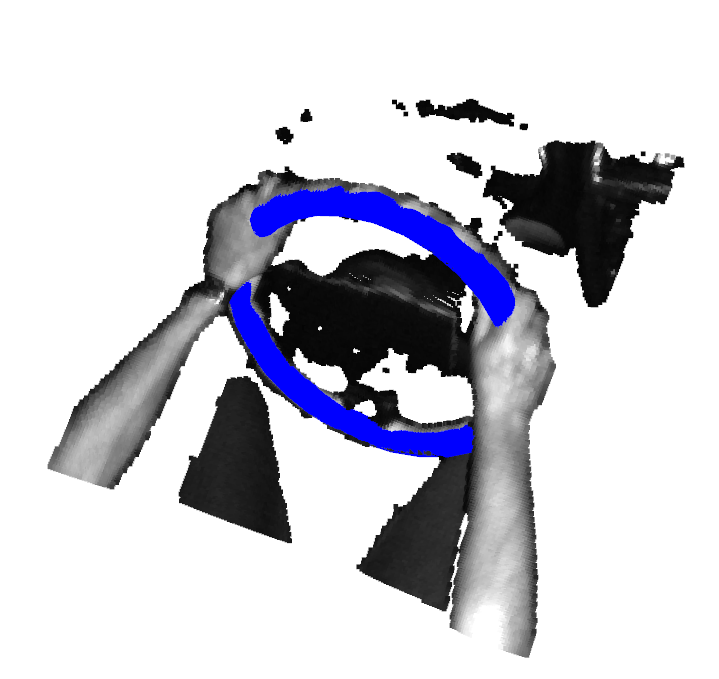
\includegraphics[width=\textwidth]{media/chapter 3/torus6.png}
    \end{subfigure}
    \caption{Torus representation of the steering wheel 
    for sample frames from the dataset}
    \label{fig:sample_toruses}
\end{figure}

\section{Ground Truth Generation: Fitting a Circle (initial approach)}

The objective of this section is to present the initial 
approach developed for generating ground truth data to 
estimate the 3D location and orientation of a steering wheel 
using 2D and 3D geometric techniques. This approach sought 
to capture the steering wheel’s geometric structure by 
fitting a 2D ellipse to the annotated points and extending this 
representation into 3D space through additional processing 
steps.


Given the complexity of manually annotating the steering wheel 
across numerous images and the inherent sparsity and noise in 
the data, the annotation process is automated and enhanced by fitting a mathematical model to a few number of spars annotations. This model would allow us to generate a 
more comprehensive representation of the steering wheel 
geometry. The approach was divided into several phases:
\begin{enumerate}
    \item Annotating the steering wheel with 2D points.
    \item Fitting an ellipse to the annotated 2D points.
    \item Sampling additional points from the ellipse and mapping them into 3D space.
    \item Fitting a sphere to the 3D points to refine the geometry.
    \item Deriving a circular cross-section from the sphere to better represent the steering wheel.
\end{enumerate}
Below, each step of this approach is explained in detail.

\subsection{Annotating the Steering Wheel with 2D Points}
The process began with manual annotation of the steering wheel 
in 2D images. Annotating a dense and accurate set of points 
across all images was infeasible due to the time-consuming 
nature of manual annotation and the large number of frames. 
Hence, a sparse set of 2D points was initially marked to 
provide a basic outline of the steering wheel as depicted in 
\cref{fig:ellipse}.

\subsection{Fitting an Ellipse to the Annotated 2D Points}
In order to create a denser representation, an ellipse was fitted to the existing 2D annotation points. This provided 
a more complete 2D shape that captured the true geometric 
structure of the steering wheel as illustrated in \cref{fig:ellipse}. 

The ellipse was fitted to these points using the general equation of an ellipse:
\[
c_0 X^2 + c_1 XY + c_2 Y^2 + c_3 X + c_4 Y = b
\]
To find the coefficients \([c_0, c_1, c_2, c_3, c_4]\) 
that best fit to the observed points \((X, Y)\), linear 
regression was applied. Defining \( A = [X^2, XY, Y^2, X, Y] \) and 
\( c = [c_0, c_1, c_2, c_3, c_4] \), the coefficients are calculated 
by solving for \( c \) that satisfies the equation \( Ac = b \), 
where \( b \) represents the constant in the ellipse equation. 


\subsection{Sampling Points from the Ellipse and Mapping to 3D}
Once the ellipse was fitted, 1000 points were sampled from 
the ellipse and its neighboring regions to create a denser 
representation as shown in \cref{fig:sampled_points}. These points were mapped from 2D to 3D using 
depth information from the camera and the intrinsic parameters.

However, due to the sparse and noisy nature of the data, 
the sampled points could not accurately represent the true 
geometry of the steering wheel, resulting in an inaccurate 
approximation of the 3D position and orientation. 
As depicted in \cref{fig:obb}, the bounding box fitted to the 
mapped 3d points was unable to accurately represent the 
position of the steering wheel.

\subsection{Fitting a Sphere to the 3D Points}
To further refine the 3D representation, a sphere was fitted to the sampled points on the steering wheel as demonstrated in
\cref{fig:sphere}. 
Given the sample points \((x, y, z)\), the general 
equation of a sphere is as following:
\[
(x - h)^2 + (y - k)^2 + (z - m)^2 = r^2
\]
Expanding this equation obtains:
\[
x^2 + h^2 - 2xh + y^2 + k^2 - 2yk + z^2 + m^2 - 2mz = r^2
\]
Rearranging terms yields:
\[
2xh + 2yk + 2zm + (r^2 - h^2 - k^2 - m^2) = x^2 + y^2 + z^2
\]
Letting \( A = [2x, 2y, 2z, 1] \), \( c = [h, k, m, r^2 - h^2 - k^2 - m^2] \), and 
\( b = x^2 + y^2 + z^2 \), a sphere can fit to the points by solving for \( c \) in the equation:
\[
Ac = b
\]

This solution provides us with the center \((h, k, m)\) and radius 
\(r\) of the sphere.


\subsection{Refining with a Circular Cross-Section from the Sphere}
To better capture the essential structure of the steering wheel, a circular cross-section of the fitted sphere in the XY plane was taken by fixing \( z = m \). This simplification was based on the observation that the steering wheel’s geometry is primarily defined in the XY plane, with minimal variation along the z-axis. 
Principal Component Analysis (PCA) of the steering wheel points 
revealed that the distribution along the z-axis is very limited, 
indicating that this axis does not contain significant information 
about the overall shape or structure of the steering wheel. 
By constraining the representation to the XY plane, unnecessary complexity from minor variations along 
the z-axis was avoided, which could detract from the accuracy of the wheel’s positioning.

This circular cross-section represented the X and Y 
correlations in the steering wheel geometry, 
simplifying the model while preserving the essential spatial 
characteristics of the wheel.


\subsection{Aligning the Circle with a Rotation Matrix}
Finally, this circle was aligned to the steering wheel’s position 
by applying a rotation matrix followed by a translation 
to center of the sphere. The rotation matrix was derived 
from the oriented bounding box of the steering wheel 3D points 
illustrated in \cref{fig:obb}. Open3D OrientedBoundingBox method 
\footnote{available at \url{http://www.open3d.org/docs/release/python_api/open3d.geometry.OrientedBoundingBox.html}}
was employed to compute the orientation and rotation matrix, 
which allowed us to align the circle with the steering 
wheel’s orientation in 3D space. 
Figure \cref{fig:circle} shows the final circular representation of the steering wheel's 3D position.

\begin{figure}[ht]
    \centering
    \begin{subfigure}[t]{0.18\textwidth}
        \centering
        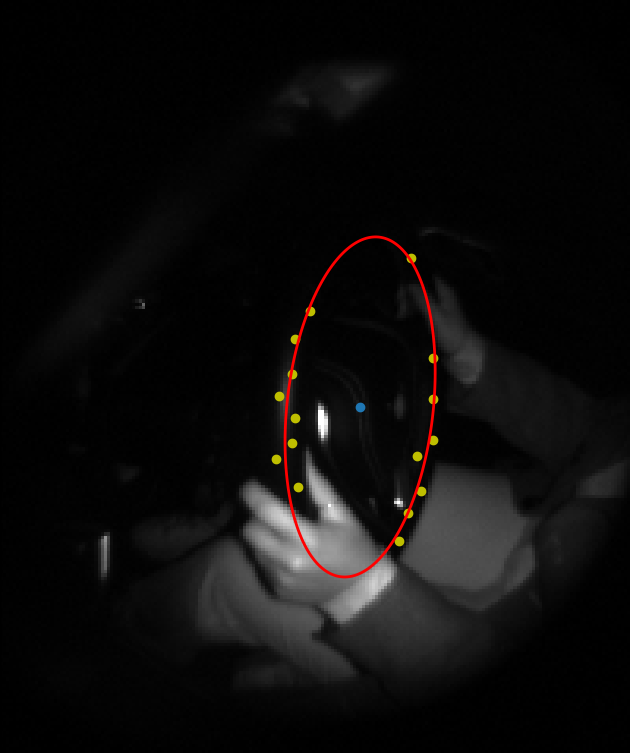
\includegraphics[width=\textwidth]{media/chapter 4/ellipse.png}
        \caption{}
        \label{fig:ellipse}
    \end{subfigure}\hfill
    \begin{subfigure}[t]{0.18\textwidth}
        \centering
        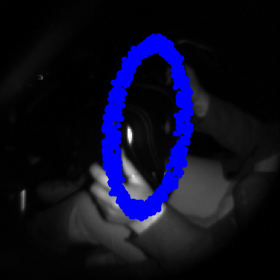
\includegraphics[width=\textwidth]{media/chapter 4/sampled_points.png}
        \caption{}
        \label{fig:sampled_points}
    \end{subfigure}\hfill
    \begin{subfigure}[t]{0.18\textwidth}
        \centering
        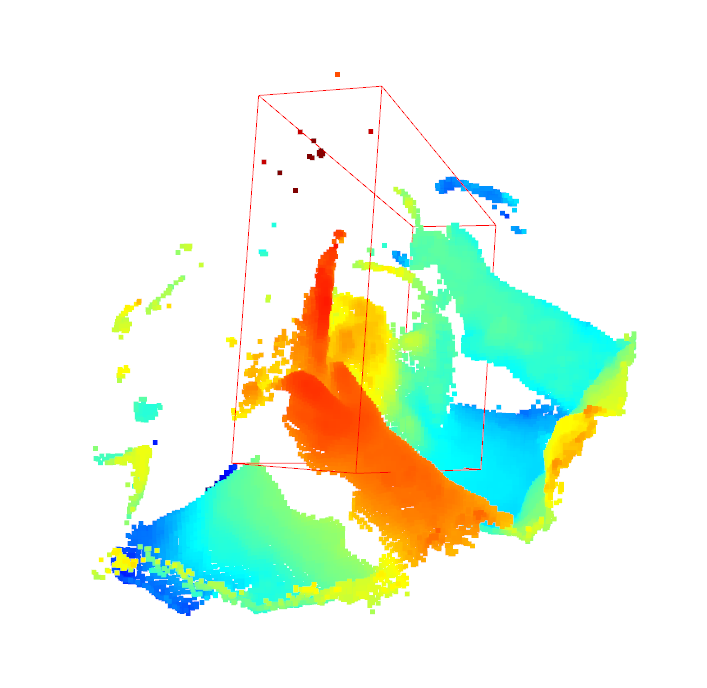
\includegraphics[width=\textwidth]{media/chapter 4/obb.png}
        \caption{}
        \label{fig:obb}
    \end{subfigure}\hfill
    \begin{subfigure}[t]{0.18\textwidth}
        \centering
        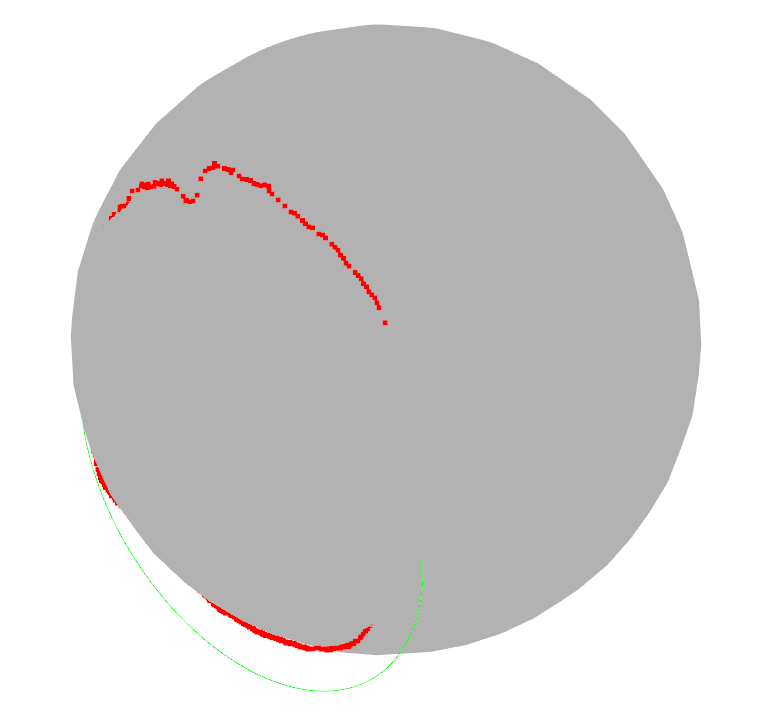
\includegraphics[width=\textwidth]{media/chapter 4/sphere.png}
        \caption{}
        \label{fig:sphere}
    \end{subfigure}\hfill
    \begin{subfigure}[t]{0.18\textwidth}
        \centering
        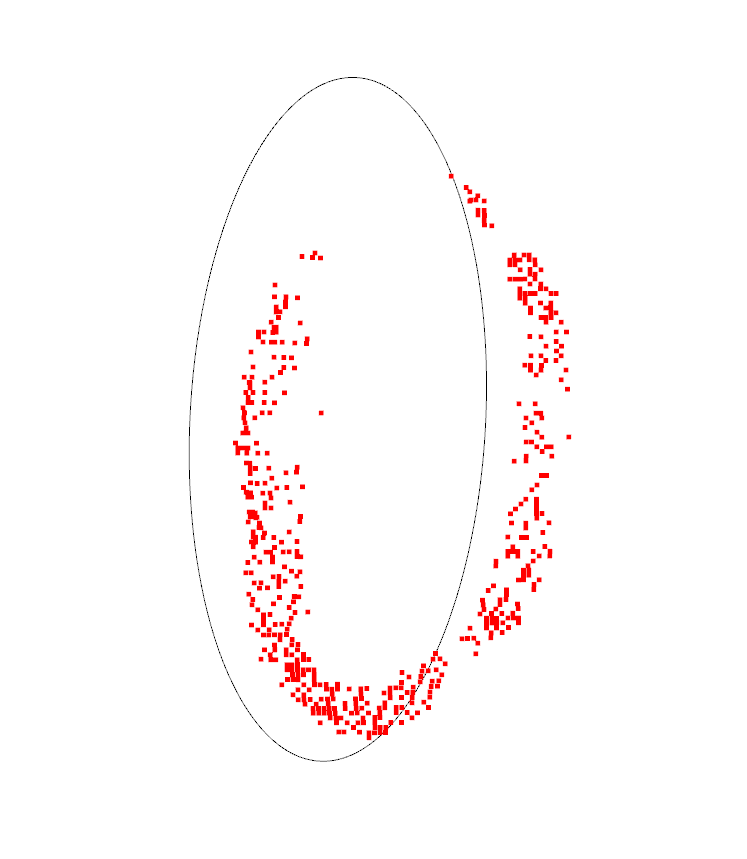
\includegraphics[width=\textwidth]{media/chapter 4/circl.png}
        \caption{}
        \label{fig:circle}
    \end{subfigure}\hfill
    \caption{(a) Steering wheel annotated with 2d points 
    and an ellipse fitted to the 2D points. (b) 1,000 points were sampled from the ellipse 
    and its small neighborhood.(c) The sampled points were mapped to 3D space, 
    with the bounding box illustrating these points in 3D. 
    (d) A sphere was fitted to the sampled points. 
    (e) The 3D model was refined by deriving a 
    circular cross-section from the sphere, representing 
    the steering wheel’s 3D position as a circle in 
    3D space.}
\end{figure}


Despite these steps, this approach was ultimately limited by the sparse and noisy data, as well as the lack of an accurate evaluation method 
for the generated ground truths. This made it difficult to ensure the 
precision of the ground truths in accurately capturing the true location and orientation of the 
steering wheel. These limitations prompted us to pursue a second 
approach using ArUco board for more reliable results.


\chapter{Ground Truth Generaiton: ArUco Markers and Plane Fitting (Refined Approach)}

\section{Introduction}
To overcome the limitations of the initial ellipse fitting 
approach, a second method was developed using ArUco markers and 
plane fitting. This method aimed to achieve precise 3D 
estimation of the steering wheel's location and orientation. 
The use of ArUco board, and a plane fitting technique allowed 
for a more robust and accurate approach to capturing the 3D 
geometry of the steering wheel. By leveraging the known 
properties and spatial relationships of the ArUco markers, 
this refined method was able to provide a reliable and 
high-quality ground truth for the steering wheel's position 
and orientation, which could then be used for training and 
evaluating 3D object detection models.


ArUco markers \cite{opencv_aruco_detection} are widely used  in 
computer vision for precise localization and pose estimation 
tasks.  An ArUco marker as depicted in \cref{fig:marker}, is a 
synthetic square marker featuring a  thick black border and an 
inner binary matrix that encodes  its identifier (ID). The black 
border enables quick detection  in images, while the binary 
matrix allows for identification  and supports error detection 
and correction.  The marker size dictates the dimensions of the 
internal matrix;  for example, a 4x4 marker contains 16 bits. 
can be easily  detected and identified in images.  They offer 
several advantages, including robustness to  variations in 
lighting, simple detection with minimal  computational overhead, 
and compatibility with popular  libraries like OpenCV, which 
provides dedicated functions for detecting ArUco markers and 
estimating their pose in both 2D  and 3D. Figures \cref{fig:marker_detection} and \cref{fig:marker_orientation} 
demonstrate OpenCV's capabilities in detecting ArUco markers and 
estimating their 3D position, respectively. 

This chapter presents the structured methodology, the evaluation 
of different techniques for location and orientation estimation, 
and the results of this second approach in accurately capturing 
the steering wheel’s 3D geometry.

\begin{figure}[ht]
    \centering
    \begin{subfigure}[t]{0.3\textwidth}
        \centering
        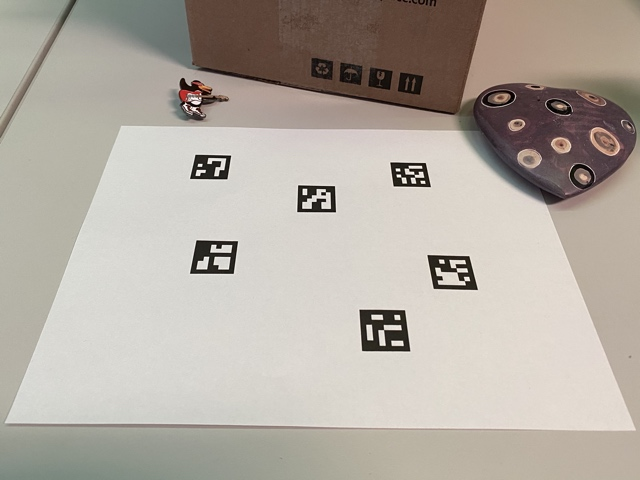
\includegraphics[width=\textwidth]{media/chapter 5/singlemarkersoriginal.jpg}
        \caption{Single ArUco Markers}
        \label{fig:marker}
    \end{subfigure}\hfill
    \begin{subfigure}[t]{0.3\textwidth}
        \centering
        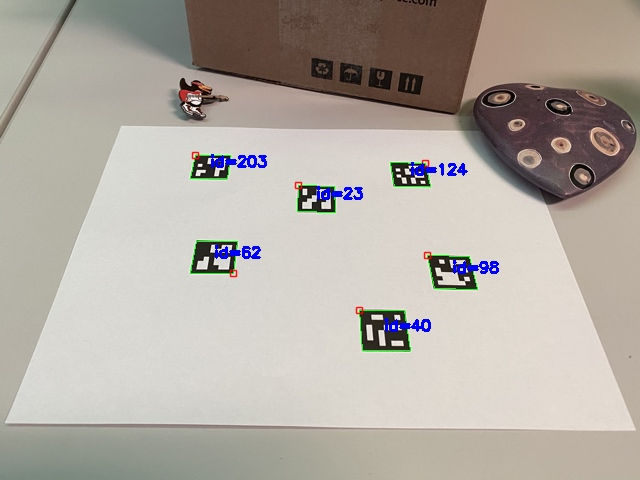
\includegraphics[width=\textwidth]{media/chapter 5/singlemarkersdetection.jpg}
        \caption{These are the detected markers (in green). 
        Note that some markers are rotated. 
        The small red square indicates the marker’s top left 
        corner}
        \label{fig:marker_detection}
    \end{subfigure}\hfill
    \begin{subfigure}[t]{0.3\textwidth}
        \centering
        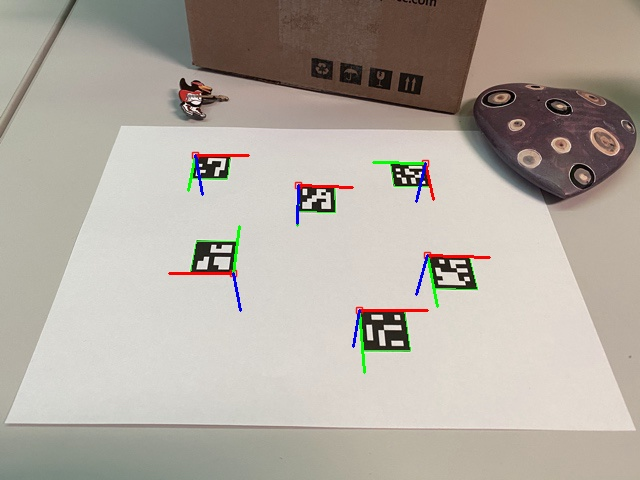
\includegraphics[width=\textwidth]{media/chapter 5/singlemarkersaxes.jpg}
        \caption{The marker coordinate system that is placed in the center or in the top left 
        corner of the marker with the Z axis pointing out. 
        Axis-color correspondences are X: red, Y: green, Z: blue.}
        \label{fig:marker_orientation}
    \end{subfigure}
    \caption{ArUco merkers' detection and pose estimation by OpenCV.}
\end{figure}

This refined approach aimed to address the challenges 
encountered in the initial method, particularly the issues of 
data sparsity, noise, and inaccurate geometric representation. 
By leveraging the advantages of ArUco markers, this method 
sought to tackle the difficulties in precisely estimating the 
3D position and orientation of the steering wheel. 

The proposed technique involved positioning a board with 
multiple ArUco markers at the center of the steering wheel 
like in \cref{fig:gt_stream} and employing plane fitting to 
enhance the accuracy of orientation estimation. 
This approach was extensively evaluated to validate its 
reliability in capturing the 3D geometry of the steering wheel.

The following sections detail 
the assessment of ArUco markers for location and orientation 
estimation, as well as the generation of the steering wheel's 
oriented bounding box using the validated methods.

\section{Methodoloy}
To address the limitations identified in the initial approach, 
a structured methodology was developed using ArUco markers and 
plane fitting. The ArUco markers were placed on a board mounted 
at the center of the steering wheel as depicted in 
\cref{fig:gt_stream}. This setup allowed us to capture both the 
2D and 3D spatial data required for accurately estimating the 
steering wheel's position and orientation.

The methodology involved two primary components for estimating 
the location and orientation of the steering wheel. 
each component is described in detail in the following 
subsections:

\subsection{location estimation}
As depicted in \cref{fig:gt_stream}, the ArUco board is positioned at the center of the steering 
wheel. Therfore, the detected centroid of the ArUco board directly 
corresponds to the 3D spatial coordinates of the steering 
wheel's center. Given the known arrangement of markers on the 
ArUco board, the location of the board's center, and 
consequently the steering wheel's center, can be readily 
inferred from the detected positions of the individual markers.

To achieve precise location estimation of the ArUco markers, 
we considered two primary approaches:

\textbf{1. Direct 3D Estimation Using OpenCV: }
OpenCV’s \emph{estimatePoseSingleMarkers} function provides a direct 
way to estimate the 3D position of markers relative to the camera. 
This function relies on the known physical size of the 
ArUco markers and the intrinsic camera parameters to calculate 
the translation vector, which represents the 3D position of 
the markers as [dx, dy, dz] where dx dy, and dz are the marker's 
position along the x, y, and z axes, respectively. 
While this method offers a straightforward approach, its 
accuracy can be sensitive to marker orientation, distance from 
the camera, and the angle of view.

\textbf{2. 2D Estimation with Mapping to 3D: }
This alternative method starts by detecting the 2D position of 
the markers in the image plane using OpenCV’s \emph{detectMarkers} 
function. \Cref{fig:detectMarkers} shows merkers' location detected 
by OpenCV on the 2D image.
After detecting the 2D positions, these points are 
mapped to 3D space using depth information derived from the 
point cloud data and the camera’s intrinsic parameters. 
This approach separates the detection process into two stages, 
potentially improving accuracy by isolating the detection of 
2D marker positions from their 3D mapping.
\begin{figure}[ht]
    \centering
    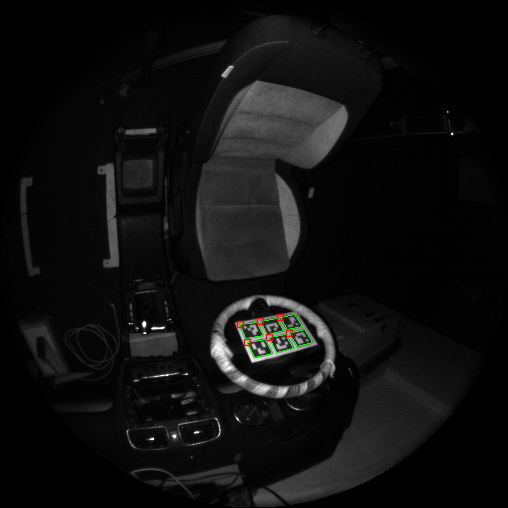
\includegraphics[scale=0.5]{media/chapter 5/aruco_detection.png}
    \caption{OpenCV detected the ArUco markers' location in the 2d image.}
    \label{fig:detectMarkers}
\end{figure}


Given the known structure and location of the markers on the board, 
we employed a method to calculate the board’s center based on the 
spatial relationship of specific marker pairs. This technique ensured 
that the center could be reliably calculated even if some markers were 
undetected.

To calculate the center of the board, we utilized three pairs of markers 
that are symmetrically positioned on opposite sides of the board as depicted
in \cref{fig:marker_ids}. These marker pairs are: \{(0, 5), (1, 4), (2, 3)\}

For each detected pair, the midpoint between the two markers was 
computed by averaging their translation vectors \( tvec \), which 
represent the 3D coordinates of each marker. This midpoint provides an 
estimate of the board’s center based on that particular pair.

For each detected pair \((i, j)\), we compute the midpoint as:
\[
\text{midpoint}_{ij} = \frac{tvec_i + tvec_j}{2}
\]

where  \(tvec_i\)  and  \(tvec_j\)  are the translation vectors 
(3D coordinates) of markers  \(i\)  and  \(j\) . Once the midpoints for 
all detected pairs are obtained, the overall center of the board is 
calculated as the mean of these midpoints:

\[
\text{center}_\text{board} = \frac{\sum{(i, j) \in \text{detected pairs}} \text{midpoint}_{ij}}{N}
\]

where  \(N\)  is the number of detected pairs. The resulting averaged 
translation vector represents the estimated 3D center of the board. 


By considering the relative positions and midpoints of detected marker 
pairs, this method can robustly determine the center point of the board, 
providing an accurate 3D location for the steering wheel despite 
potential occlusions or missing markers.

\begin{figure}[ht]
    \centering
    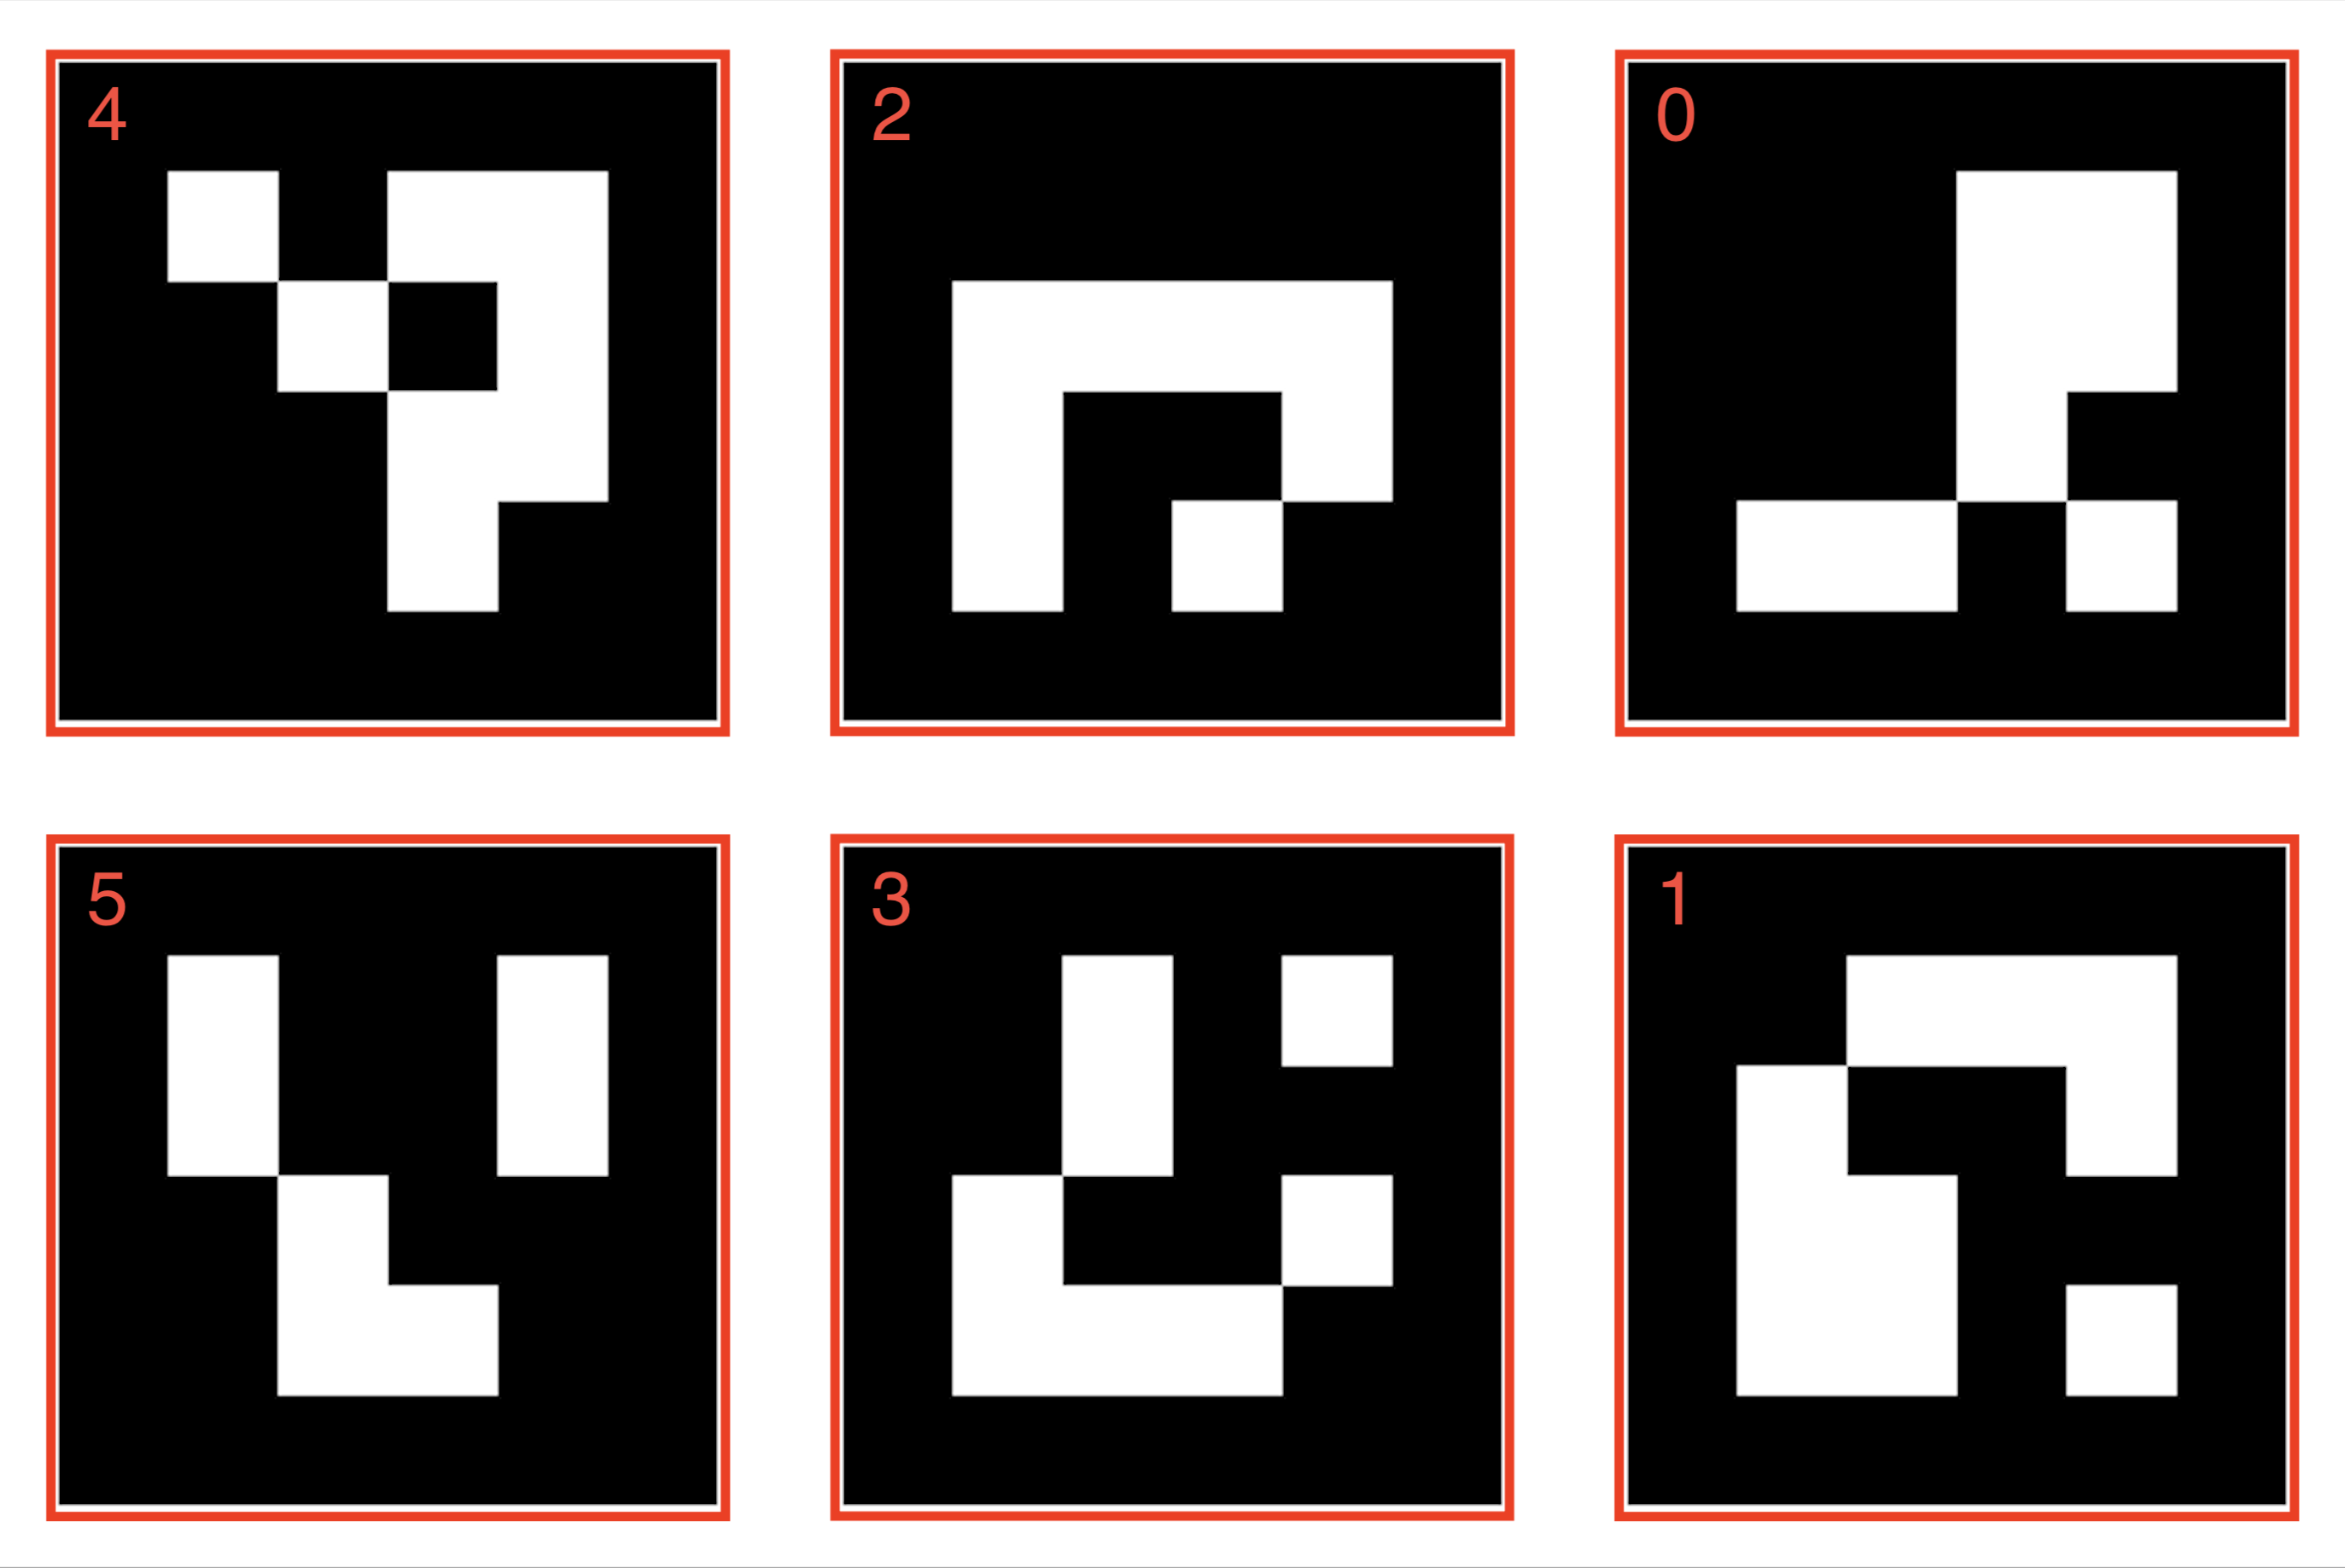
\includegraphics[scale=0.5]{media/chapter 5/aruco_board_ids.png}
    \caption{To calculate the center of the board, we utilized multiple 
    marker pairs that are symmetrically positioned on opposite sides of 
    the board as marker pairs \{(0,5), (1,4), (2,3)\}.}
    \label{fig:marker_ids}
\end{figure}


\subsection{Evaluating ArUco Markers for Orientation Estimation}
Accurately determining the orientation of the marker board was 
critical for estimating the steering wheel’s orientation. 
As the ArUco board is accurately placed tangent to the steering 
wheel, the orientation of the board corresponds to the 
orientation of the steering wheel in 3D space. 

Two methods were used exploited to estimate the orientation of 
the ArUco board: 

\uzlemph{Direct Orientation Estimation Using OpenCV: }
OpenCV’s \emph{estimatePoseSingleMarkers} function also calculates the 
orientation of markers in the form of rotation vectors. 
These vectors indicate the rotational pose of each marker 
relative to the camera’s coordinate system. Assuming the we 
know the  orientation of the markers on the board, we can 
remove the outlier markers and average the remaining rotation 
vectors to estimate the overall orientation of the board.
However, this method has limitations, as it relies on the 
accuracy of OpenCV's built-in pose estimation.

As illustrated in \cref{fig:estimatePoseSingleMarkers}, 
OpenCV's estimations of marker 
positions on a 3×4 board are highly sensitive to several factors. 
These include the camera angle, the distance of the markers from 
the camera, occlusion of the markers, and other environmental 
factors. Consequently, when markers are missing or occluded, 
the reliability and accuracy of the orientation estimation can 
decrease significantly. This sensitivity to various spatial and 
environmental conditions highlights the limitations of relying 
solely on OpenCV's built-in pose estimation functions for robust 
3D orientation determination.

\begin{figure}[ht]
    \centering
    \begin{subfigure}[t]{0.23\textwidth}
        \centering
        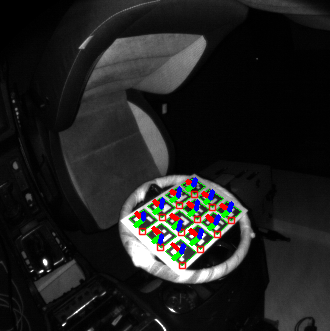
\includegraphics[width=\textwidth]{media/chapter 5/aruco_board_estimation0.png}
    \end{subfigure}\hfill
    \begin{subfigure}[t]{0.23\textwidth}
        \centering
        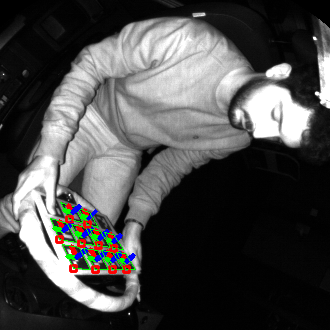
\includegraphics[width=\textwidth]{media/chapter 5/aruco_board_estimation1.png}
    \end{subfigure}\hfill
    \begin{subfigure}[t]{0.23\textwidth}
        \centering
        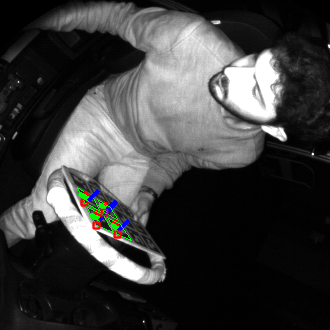
\includegraphics[width=\textwidth]{media/chapter 5/aruco_board_estimation2.png}
    \end{subfigure}\hfill
    \begin{subfigure}[t]{0.23\textwidth}
        \centering
        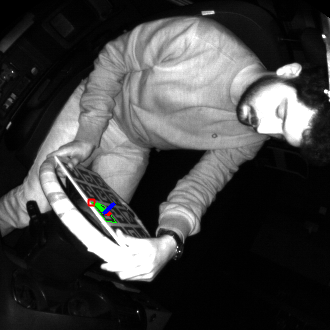
\includegraphics[width=\textwidth]{media/chapter 5/aruco_board_estimation3.png}
    \end{subfigure}
    \caption{The markers' coordinate system estimated by OpenCV's
            \emph{estimatePoseSingleMarkers} function on a 3x4
            board shows that this method is highly sensitive
            to the markers' distance, camera angle and other
            environmental factors. Axis-color correspondences are 
            X: red, Y: green, Z: blue, with Z axis pointing out}
    \label{fig:estimatePoseSingleMarkers}
\end{figure}

\uzlemph{Plane Fitting Method: }
The plane fitting method provided a more robust and reliable 
means of estimating the orientation, as it doesn't depend solely 
on the accuracy of OpenCV's pose estimation for individual 
markers. This approach overcomes the limitations of the direct 
orientation estimation using OpenCV, which can be sensitive to 
factors like marker size, distance, and viewing angle. 
Hence, the plane fitting method offers a more stable and 
accurate estimate of the steering wheel's orientation under a 
variety of conditions.

This method involves the following steps:

\begin{enumerate}
    \item \emph{Finding the Center of the ArUco Board: }
    To initiate plane fitting, it is essential to first locate 
    the center of the ArUco board. This is done using the 
    detected marker locations. Given that the markers are 
    arranged in a known, fixed structure on the board, 
    the center can be reliably estimated even if one or more 
    markers are not detected. By analyzing the relative 
    positions of the detected markers, the center of the board 
    can be computed with high accuracy.
    \item \emph{Sampling Points Around the Center: }
    Once the center of the ArUco board is determined, 
    a set of points is sampled from the board around this 
    central point within a specified radius. This sampling 
    process ensures that the points used for plane fitting are 
    well-distributed across the board, enhancing the reliability 
    of the orientation estimation. \Cref{fig:plane_fitting} shows 
    the sampled points from the board in red.
    \item \emph{Fitting a Plane to the Sampled Points: }
    The sampled points are then used to fit a plane. 
    The fitting process involves computing the best-fit plane 
    that minimizes the distance between the plane and the 
    sampled points. This plane effectively represents the 
    overall orientation of the ArUco board.
    \item \emph{Using the Normal Vector for Orientation: }
    The normal vector of the fitted plane is then calculated. 
    This normal vector serves as a robust indicator of 
    the board’s orientation in 3D space. As \cref{fig:plane_fitting}
    shows, the light blue line indicated the norm vector of the board.
    Since the board is mounted on the steering wheel tangent to the 
    steering wheel's surface, the orientation of this normal vector 
    directly corresponds to the orientation of the steering wheel.
\end{enumerate}

\begin{figure}[ht]
    \centering
    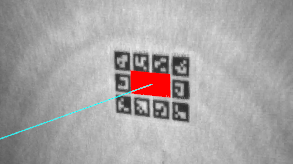
\includegraphics[width=0.5\textwidth]{media/chapter 5/plane_fitting.png}
    \caption{Illustration of the plane fitting method, showing the 
    sampled points around the center of the ArUco board in red and the 
    normal vector of the fitted plane in light blue, which represents 
    the orientation of the steering wheel.}
    \label{fig:plane_fitting}
\end{figure}

One of the significant advantages of this method is its 
robustness to marker detection failures. Even if some markers 
are not detected due to occlusions, lighting conditions, or 
other factors, the known arrangement of the markers allows for 
accurate estimation of the board’s center and subsequent 
orientation. This makes the plane fitting method highly 
resilient to errors in individual marker detections, ensuring 
reliable orientation estimation under a variety of conditions.


\subsection{Generating the Steering Wheel’s Oriented Bounding Box}
\section{Results}
\subsection{Location Estimation Results}
\uzlemph{Inter-Marker Distance Evaluation}
\uzlemph{Distance and Angle Variation}
\subsection{Orientation Estimation Results}
\
\subsection{Systematic Error in Orientation Estimation}
\subsection{Generating the Steering Wheel’s Oriented Bounding Box}

\section{Conclusion}
\chapter{Model and Methodology}
\section{Introduction}
This chapter presents the approach adopted to estimate the 3D position and orientation of the steering wheel using 3D point clouds. Based on Voxel R-CNN \cite{voxelrcnn}, a voxel-based 3D object detection framework, our methodology includes specific modifications to account for the steering wheel’s unique characteristics, including adjustments to bounding box encodings and adaptations for SWD-dataset cubic point clouds. The chapter first provides an overview of Voxel R-CNN’s architecture, then delves into the modifications made to accommodate steering wheel detection.


\section{Network Architecture}
Voxel R-CNN framework, a two-stage voxel-based architecture for 3D object detection. As illustrated in \cref{fig:voxelrcnn}, Voxel R-CNN comprises several key components: a 3D backbone network, a 2D backbone network followed by a Region Proposal Network, and a voxel RoI pooling module coupled with a detection subnet for box refinement. The approach begins by dividing the input point cloud into regular voxels and utilizing the 3D backbone network to extract features from this voxelized representation. These sparse 3D voxel features are then converted into a Bird's Eye View representation, on which the 2D backbone network and RPN are applied to generate 3D region proposals. Finally, the voxel RoI pooling module is used to extract region-specific features, which are then fed into the detection subnet for further refinement of the bounding box predictions. The following sections provide a more detailed discussion of these individual modules, with a particular focus on the innovative voxel RoI pooling component.

\begin{figure}[htpb]
    \centering
    \includegraphics[width=\textwidth]{media/chapter 6/voxelrcnn2.png}
    \caption{Voxel R-CNN pipeline: The input point cloud is voxelized, and features are extracted using a 3D backbone network. These features are transformed into a Bird’s Eye View and processed by a 2D backbone and Region Proposal Network (RPN) to generate 3D region proposals. Finally, voxel RoI pooling extracts region-specific features for box refinement in the detection subnet.}
    \label{fig:voxelrcnn}
\end{figure}

\subsection{Voxel Feature Encoding (VFE)}
The VFE module extracts relevant features from the individual points within each voxel, such as 3D coordinates, intensity, and other attributes. This helps the network understand the spatial structure and density of the point cloud in that region.

After extracting the point-wise features, the VFE module aggregates them into a single feature vector representing the entire voxel. This aggregation typically uses pooling operations like max pooling or mean pooling to summarize the information across all points. The resulting compact, fixed-size feature representation is essential for efficiently processing the voxel grid in the subsequent 3D convolutional layers, allowing the network to focus on meaningful spatial features without being overwhelmed by the raw data's sparsity and variability.

\subsection{3D Backbone}
The 3D backbone in Voxel R-CNN is a crucial component that processes the structured voxel feature map produced by the VFE module. This backbone network typically consists of a series of 3D convolutional layers that operate on the voxelized input, allowing the model to learn complex spatial patterns and relationships in 3D space. By applying 3D convolutions, the backbone captures both local and global context within the point cloud, identifying meaningful features across the x, y, and z dimensions. 

The backbone network usually follows a hierarchical structure, similar to standard CNNs, where initial layers capture low-level details, and deeper layers extract high-level, abstract features. There are three stages in the 3D back-bone with filter numbers of 16,32,64 respectively. This layered approach enables the backbone to detect small, local structures in the early stages and progressively combine them into larger, more meaningful shapes or object parts. After passing through the backbone, the 3D voxel features are transformed into a feature representation that is both spatially compact and semantically rich, making it suitable for downstream tasks like region proposal generation and bounding box prediction. Overall, the 3D backbone enhances Voxel R-CNN's ability to detect and classify objects in cluttered and complex 3D environments by learning a comprehensive representation of the spatial layout.

\subsection{Bird's Eye View Transformation}
The Bird's Eye View module in Voxel R-CNN converts 3D spatial features into a 2D representation from a top-down viewpoint. This process simplifies the 3D data by collapsing the height dimension. The BEV module concentrates on the x-y plane, retaining crucial spatial relationships. By aggregating voxel features along the z-axis, the BEV module creates a compact 2D feature map that reduces computational complexity while preserving spatial information. This 2D representation can then be efficiently processed using 2D convolutional techniques for tasks like region proposal and bounding box regression, enabling faster inference and alignment with real-time requirements in autonomous driving applications.

\subsection{2D Backbone}
The 2D backbone in Voxel R-CNN is designed to extract and refine features from the Bird’s Eye View (BEV) feature map, optimizing the network’s understanding of object locations in the x-y plane. This backbone consists of two main components: a top-down feature extraction sub-network and a multi-scale feature fusion sub-network.

The top-down feature extraction sub-network is composed of two blocks of standard 3×3 convolutional layers, which are crucial for capturing spatial details and patterns in the BEV representation. The first block maintains the same resolution as the 3D backbone’s output along the x and y axes, ensuring alignment with the original spatial layout. The second block operates at half the resolution of the first, capturing more abstract and larger-scale features. Each block contains 5 convolutional layers, with feature dimensions set to 64 and 128, respectively, allowing for a progressively richer feature representation.

Following feature extraction, the multi-scale feature fusion sub-network performs upsampling and concatenation of these top-down features, merging information across scales. This fusion process enables the 2D backbone to integrate fine-grained details with broader contextual information, enhancing its ability to recognize objects and understand their spatial relationships. Together, these components provide a robust feature map, which supports effective object detection and localization in the BEV space, while maintaining computational efficiency.


\subsection{Region Proposal Network (RPN)}
Region Proposal Network (RPN) module in Voxel R-CNN is responsible for generating candidate regions, or proposals, where objects are likely located within the Bird’s Eye View (BEV) feature map. This module plays a critical role in reducing the search space for the detection network by focusing on areas that are more likely to contain objects, rather than examining the entire feature map exhaustively.

The RPN works by sliding a small network over the BEV feature map output from the 2D backbone. For each location in the feature map, the RPN proposes bounding boxes with different sizes and aspect ratios, known as anchors, which act as initial guesses for potential object locations. The RPN then evaluates each anchor’s likelihood of containing an object by assigning objectness scores, as well as refining the bounding box coordinates through regression. Anchors with high objectness scores are selected as region proposals and are further refined to improve localization accuracy.

Once the RPN generates these proposals, they are used as input for the subsequent detection head, where they undergo further processing to classify objects and predict precise 3D bounding boxes. This selective proposal approach improves computational efficiency by allowing the detection network to focus on fewer, relevant regions rather than processing the entire scene. The RPN thus enables Voxel R-CNN to perform object detection with greater speed and accuracy, a necessity for real-time autonomous driving applications.

\subsection{RoI Head}
In Voxel R-CNN, \emph{Voxel RoI Pooling} is a specialized operation designed to handle sparse 3D feature volumes efficiently. Unlike traditional RoI pooling, where max pooling is applied over regular grid points, Voxel RoI pooling accounts for the sparse nature of 3D voxel data, as less than 3\% of the 3D space typically contains non-empty voxels. The Voxel RoI pooling layer starts by dividing each region proposal into a grid of \(6 \times 6 \times 6\) sub-voxels. For each sub-voxel, the grid point at its center is selected as the reference for feature extraction.

Since max pooling over each sub-voxel isn’t feasible in sparse data, Voxel RoI pooling uses a \emph{neighboring voxel aggregation approach}. As depictred in \cref{fig:roi_pooling}, for each grid point \(g_i\), a set of neighboring voxels, \(\Gamma_i = \{v_i^1, v_i^2, \ldots, v_i^K\}\), is identified using a \emph{voxel query} presented by Deng et al. \cite{voxelrcnn} . Then, the features from these neighboring voxels are aggregated using a \emph{PointNet module}. A max pooling operation over the channels then produces an aggregated feature vector \(\eta_i\) for each grid point, summarizing the features of nearby voxels. To capture multi-scale features, Voxel RoI pooling extracts voxel features from the final two stages of the 3D backbone network using different distance thresholds for each stage, allowing it to concatenate multi-scale RoI features.

\begin{figure}[htpb]
    \centering
    \includegraphics[width=0.5\textwidth]{media/chapter 6/roi_pooling.png}
    \caption{Voxel RoI pooling aggregates features from neighboring voxels for each grid point \(g_i\) using a voxel query approach \cite{voxelrcnn}, then applies a PointNet module followed by max pooling to produce an aggregated feature vector \(\eta_i\), summarizing local voxel features. Source: \cite{voxelrcnn}}
    \label{fig:roi_pooling}
\end{figure}

Once RoI features are extracted, they are passed to the \emph{detection head} for further refinement and prediction. This detection head takes the RoI features and first transforms them into feature vectors via a shared 2-layer MLP. The output is then split into two branches: a \emph{bounding box regression branch} and a \emph{confidence prediction branch}. The box regression branch refines the bounding box coordinates by predicting the residuals from the region proposals to the ground truth boxes, ensuring precise localization. The confidence prediction branch, on the other hand, outputs an IoU-related confidence score that represents the likelihood of the proposal being a correctly localized object. Together, these two branches allow the detection head to generate highly accurate 3D bounding boxes and confidence scores for each detected object.

These blocks collectively enable Voxel R-CNN to balance high-speed processing with accurate 3D object detection by capitalizing on voxel-based representations.


\section{Adaptatoins for steering wheel detection}
This section outlines the series of modifications and methodological adaptations made to the Voxel R-CNN model to suit the specific needs of steering wheel detection in the SWD dataset. While Voxel R-CNN was initially developed for general 3D object detection tasks in autonomous driving, the unique characteristics of steering wheel detection required focused changes to both the bounding box encoding, some utility functions and model structure.

The modifications began with redefining the bounding box encoding to align with the steering wheel’s primary orientation changes along the x-axis. Next, the 3D backbone network was refined to accommodate the cubic structure of the SWD dataset’s point clouds, ensuring the model retained detail across all spatial dimensions.

Together, these modifications enabled Voxel R-CNN to function effectively within the context of steering wheel detection, capturing the steering wheel’s orientation and position with high accuracy.

\subsection{Adjustments to Bounding Box Encodings}
Although the SWD dataset provides ground truth bounding boxes with three degrees of freedom (DOF) for rotation—capturing orientation in all three axes \((x, y, z)\)—Voxel R-CNN’s architecture is limited in handling multiple rotation axes due to its original design constraints, which encode bounding boxes with only one rotational DOF.



In adapting the SWD dataset for Voxel R-CNN, the x-axis was prioritized for bounding box rotation. Unlike general 3D objects, the steering wheel’s primary rotational adjustments occur along the x-axis, which corresponds to tilting or adjusting the wheel’s angle toward or away from the driver. Given Voxel R-CNN’s single-degree-of-freedom (DOF) limitation in encoding rotation, focusing on the x-axis allowed us to capture the most relevant orientation data for the steering wheel’s positioning without introducing unnecessary complexity. 



The SWD dataset provides ground truth bounding boxes with an extended encoding format: \([x, y, z, dx, dy, dz, ax, ay, az]\), where \((ax, ay, az)\) represent the angles between the steering wheel’s normal vector and the camera’s coordinate axes.
To adapt this encoding for Voxel R-CNN, the bounding box format was modified to focus on rotation along the x-axis. Specifically, the rotation angle \(rx\) was calculated as:
\[
rx = -\arctan\left(\cos(az), \cos(ay)\right)
\]


The adapted bounding box format for this model thus became \([x, y, z, dx, dy, dz, rx]\), with rx encoding the rotation around the x-axis. This modification enabled Voxel R-CNN to accurately interpret the orientation of the steering wheel in a manner consistent with the dataset’s ground truth annotations.


However, considering only a single DOF meant that the ground truth bounding boxes no longer fully encapsulated the entire steering wheel due to its circular shape and orientation variability. To address this, bounding box dimensions were adjusted by doubling the bounding box length along the \(z\) axis (toward the steering wheel) to ensure the entire steering wheel remained within the bounding box despite the rotational limitation. This modification enabled Voxel R-CNN to provide comprehensive spatial coverage of the steering wheel while adhering to its single DOF encoding constraint.



Adapting the rotation axis required modifying several internal functions. First, the rotation calculations were changed to work with the x-axis rotation, rather than the original z-axis approach. This ensured the model correctly interpreted the steering wheel's orientation. Additionally, the 2D and 3D Intersection over Union metrics, used to evaluate bounding box accuracy, was updated to compare boxes based on the new x-axis rotation encoding. These modifications maintained consistency and precision throughout the detection process.


\subsection{Network Adjustments}
In this work, the 3D backbone network were modified to accommodate cubic point clouds, differing from the original Voxel R-CNN setup designed for elongated voxel grids. The SWD dataset used here spans a fixed range of [-0.167, 0.333] meters along the x-axis, [-0.01, 0.49] meters along the y-axis, and [0.438, 0.938] meters along the z-axis. Given a voxel size of 0.002 meters, this results in a voxel grid of 250\times250\times250 \((x, y, z)\), producing a cubic representation with uniform resolution across all three spatial dimensions.


In contrast, the original Voxel R-CNN backbone configuration, designed for the KITTI dataset, utilizes a voxel grid with unbalanced dimensions, such as 1408\times1600\times80. This elongated grid reflects KITTI’s larger coverage along the \(x\) and \(y\) axes, while the z-axis covers a relatively limited vertical range, leading to a structure optimized for road-level scenes but not ideal for cubic point clouds.


To adapt Voxel R-CNN for the SWD dataset, the 3D backbone network’s stages reduced to 3 with filter counts of 16, 32, and 64 in each stage respectively. The overall stride of the 3D backbone is set to 8. Consequently, the initial 250\times250\times250 voxel grid is downsampled to a final output resolution of 32\times32\times32. This balanced reduction preserves spatial consistency across all dimensions, which is critical for cubic datasets like SWD.

These backbone adjustments allow the network to effectively capture object features within the cubic point cloud, maintaining spatial fidelity that supports accurate detection in applications requiring uniform voxelization

\section{Summary}
In summary, this chapter detailed the modifications made to Voxel R-CNN to suit the steering wheel detection task. By altering the bounding box encodings to capture relevant x-axis rotation, adapting SWD dataset ground truths, and balancing feature extraction for cubic point clouds, Voxel R-CNN were optimized for accurate and efficient steering wheel detection within a 3D space.
\chapter{discussion}
\chapter{Conclusion}

This thesis presented a novel approach for detecting and localizing the steering wheel within 3D point clouds, specifically addressing the challenges of in-cabin automotive monitoring. The research contributed two primary innovations: the creation of the SWD dataset, capturing detailed 3D spatial representations of steering wheel positions, and the adaptation of the Voxel R-CNN model to meet the unique requirements of steering wheel detection. Together, these efforts have enabled precise and reliable estimation of both the 3D position and orientation of the steering wheel, a critical step for enhancing in-cabin monitoring and driver-assist systems.

The creation of the SWD dataset, with its tailored recording setup and structured marker arrangement, established a robust foundation for training and evaluation. The dataset’s comprehensive coverage across various angles, positions, and driver interactions provided a challenging yet realistic environment for testing detection capabilities in confined spaces. Through custom data preprocessing, such as distortion correction and noise reduction, the dataset facilitated precise ground truth generation, ensuring accuracy in evaluating the model’s spatial understanding.

Adapting Voxel R-CNN to this task involved several key modifications, including adjusting bounding box encoding to prioritize x-axis rotation and customizing the model’s 3D backbone to handle cubic point clouds effectively. These modifications addressed the specific spatial and rotational characteristics of the steering wheel, resulting in high recall and precision in detecting the steering wheel across 3D and Bird’s Eye View (BEV) projections. Evaluation metrics further validated the model’s performance, with high mAP scores, low distance error, and minimal rotation error confirming the model’s robustness in both positioning and orientation estimation.

The results of this research demonstrate the feasibility of deploying 3D object detection for in-cabin applications, particularly in scenarios where accurate steering wheel tracking is essential. The model’s ability to generalize across a variety of perspectives and orientations underscores its potential for practical use in automotive settings, contributing to safety and monitoring systems. The findings of this thesis not only highlight the adaptability of Voxel R-CNN but also lay a foundation for further advancements in 3D in-cabin monitoring.

In conclusion, this thesis provides a comprehensive approach to steering wheel detection using 3D point clouds, paving the way for enhanced in-cabin monitoring solutions. The advancements achieved here form a valuable basis for future research and application in autonomous driving and driver-assistive technology, where precise spatial awareness of in-cabin elements is increasingly vital.ß
% Normally, the bibliography comes next at this point. Do *not* (try
% to) include further indices and tables like an index or
% a list of figures or a list of tables or such things. Nobody
% actually uses them and they just use up space. 
%
% You *can* however include a glossary, if this seems appropriate. It
% goes here as an unnumbered chapter. Most thesis will *not* need a
% glossary: a well-written text (re)explains strange words and
% concepts as necessary. However, there are situations where a
% glossary may be helpful.

\begin{bibtex-entries}

@misc{stereo_rcnn,
author = {Peiliang Li AND Xiaozhi Chen AND Shaojie Shen},
title = {Stereo R-CNN Based 3D Object Detection for Autonomous Driving},
year = {2019},
month = {06},
doi = {10.1109/cvpr.2019.00783},
url = {https://doi.org/10.1109/cvpr.2019.00783}
}
@misc{pseudo_lidar,
author = {Yan Wang AND Wei‐Lun Chao AND Divyansh Garg AND Bharath Hariharan AND Mark Campbell AND Kilian Q. Weinberger},
title = {Pseudo-LiDAR From Visual Depth Estimation: Bridging the Gap in 3D Object Detection for Autonomous Driving},
year = {2019},
month = {06},
doi = {10.1109/cvpr.2019.00864},
url = {https://doi.org/10.1109/cvpr.2019.00864}
}
@misc{pseudo_lidar++,
author = {Yurong You AND Yan Wang AND Wei‐Lun Chao AND Divyansh Garg AND Geoff Pleiss AND Bharath Hariharan AND Mark Campbell AND Kilian Q. Weinberger},
title = {Pseudo-LiDAR++: Accurate Depth for 3D Object Detection in Autonomous Driving},
journal = {Cornell University},
year = {2019},
month = {01},
doi = {10.48550/arxiv.1906.06310},
url = {https://arxiv.org/abs/1906.06310}
}
@article{dsgn,
author = {Yilun Chen AND Shu Liu AND Xiaoyong Shen AND Jiaya Jia},
title = {DSGN: Deep Stereo Geometry Network for 3D Object Detection},
year = {2020},
month = {06},
doi = {10.1109/cvpr42600.2020.01255},
url = {https://doi.org/10.1109/cvpr42600.2020.01255}
}
@article{voxelnet,
  author       = {Yin Zhou and
                  Oncel Tuzel},
  title        = {VoxelNet: End-to-End Learning for Point Cloud Based 3D Object Detection},
  journal      = {CoRR},
  volume       = {abs/1711.06396},
  year         = {2017},
  url          = {http://arxiv.org/abs/1711.06396},
  eprinttype    = {arXiv},
  eprint       = {1711.06396},
  timestamp    = {Mon, 13 Aug 2018 16:46:15 +0200},
  biburl       = {https://dblp.org/rec/journals/corr/abs-1711-06396.bib},
  bibsource    = {dblp computer science bibliography, https://dblp.org}
}
@article{voxelrcnn,
author = {Jiajun Deng AND Shaoshuai Shi AND Peiwei Li AND Wengang Zhou AND Yanyong Zhang AND Houqiang Li},
title = {Voxel R-CNN: Towards High Performance Voxel-based 3D Object Detection},
journal = {Association for the Advancement of Artificial Intelligence},
volume = {35},
number = {2},
pages = {1201-1209},
year = {2021},
month = {05},
doi = {10.1609/aaai.v35i2.16207},
url = {https://doi.org/10.1609/aaai.v35i2.16207}
}
@article{se_ssd,
author = {Zheng Wu AND Weiliang Tang AND Li Jiang AND Chi‐Wing Fu},
title = {SE-SSD: Self-Ensembling Single-Stage Object Detector From Point Cloud},
year = {2021},
month = {06},
doi = {10.1109/cvpr46437.2021.01426},
url = {https://doi.org/10.1109/cvpr46437.2021.01426}
}
@article{bdc_det,
author = {Qiangeng Xu AND Yiqi Zhong AND Ulrich Neumann},
title = {Behind the Curtain: Learning Occluded Shapes for 3D Object Detection},
journal = {Association for the Advancement of Artificial Intelligence},
volume = {36},
number = {3},
pages = {2893-2901},
year = {2022},
month = {06},
doi = {10.1609/aaai.v36i3.20194},
url = {https://doi.org/10.1609/aaai.v36i3.20194}
}
@misc{point_rcnn,
author = {Shaoshuai Shi AND Wei Wang AND Hongsheng Li},
title = {PointRCNN: 3D Object Proposal Generation and Detection from Point Cloud},
journal = {Cornell University},
year = {2018},
month = {01},
doi = {10.48550/arxiv.1812.04244},
url = {https://arxiv.org/abs/1812.04244}
}
@misc{point_gnn,
author = {Weijing Shi AND  Ragunathan AND  Rajkumar},
title = {Point-GNN: Graph Neural Network for 3D Object Detection in a Point Cloud},
journal = {Cornell University},
year = {2020},
month = {01},
doi = {10.48550/arxiv.2003.01251},
url = {https://arxiv.org/abs/2003.01251}
}
@misc{pointnet++,
author = {Charles R. Qi AND Yi Li AND Hao Su AND Leonidas Guibas},
title = {PointNet++: Deep Hierarchical Feature Learning on Point Sets in a Metric Space},
journal = {Cornell University},
year = {2017},
month = {01},
doi = {10.48550/arxiv.1706.02413},
url = {https://arxiv.org/abs/1706.02413}
}
@article{pv_rcnn,
author = {Shaoshuai Shi AND Chaoxu Guo AND Li Jiang AND Zhe Wang AND Jianping Shi AND Wei Wang AND Hongsheng Li},
title = {PV-RCNN: Point-Voxel Feature Set Abstraction for 3D Object Detection},
year = {2020},
month = {06},
doi = {10.1109/cvpr42600.2020.01054},
url = {https://doi.org/10.1109/cvpr42600.2020.01054}
}
@article{pointpainting,
author = {Sourabh Vora AND Alex Lang AND Bassam Helou AND Oscar Beijbom},
title = {PointPainting: Sequential Fusion for 3D Object Detection},
year = {2020},
month = {06},
doi = {10.1109/cvpr42600.2020.00466},
url = {https://doi.org/10.1109/cvpr42600.2020.00466}
}

@article{frustum_pointnet,
  author       = {Charles Ruizhongtai Qi and
                  Wei Liu and
                  Chenxia Wu and
                  Hao Su and
                  Leonidas J. Guibas},
  title        = {Frustum PointNets for 3D Object Detection from {RGB-D} Data},
  journal      = {CoRR},
  volume       = {abs/1711.08488},
  year         = {2017},
  url          = {http://arxiv.org/abs/1711.08488},
  eprinttype    = {arXiv},
  eprint       = {1711.08488},
  timestamp    = {Wed, 11 Nov 2020 08:48:10 +0100},
  biburl       = {https://dblp.org/rec/journals/corr/abs-1711-08488.bib},
  bibsource    = {dblp computer science bibliography, https://dblp.org}
}

@misc{avod,
author = {Jason S. Ku AND Melissa Mozifian AND Jungwook Lee AND Ali Harakeh AND Steven L. Waslander},
title = {Joint 3D Proposal Generation and Object Detection from View Aggregation},
year = {2018},
month = {10},
doi = {10.1109/iros.2018.8594049},
url = {https://doi.org/10.1109/iros.2018.8594049}
}

@misc{mv3d,
author = {Chen; Xiaozhi; Ma; Huimin; Wan; Ji; Li; Bo; Xia; Tian undefined},
title = {Multi-View 3D Object Detection Network for Autonomous Driving},
year = {2016},
month = {11},
url = {https://arxiv.org/abs/1611.07759v2}
}

@article{survey,
author = {Eduardo Arnold AND Omar Y. Al-Jarrah AND Mehrdad Dianati AND Saber Fallah AND David Oxtoby AND Alex Mouzakitis},
title = {A Survey on 3D Object Detection Methods for Autonomous Driving Applications},
journal = {Institute of Electrical and Electronics Engineers},
volume = {20},
number = {10},
pages = {3782-3795},
year = {2019},
month = {01}
}

@article{kitti,
  author = {Andreas Geiger and Philip Lenz and Christoph Stiller and Raquel Urtasun},
  title = {Vision meets Robotics: The KITTI Dataset},
  journal = {International Journal of Robotics Research (IJRR)},
  year = {2013}
}

@misc{nuscenes,
author = {Holger Caesar AND Varun Bankiti AND Alex Lang AND Sourabh Vora AND Venice Erin Liong AND Qiang Xu AND Krishnan Anush AND Pan Yu AND Giancarlo Baldan AND Oscar Beijbom},
title = {nuScenes: A multimodal dataset for autonomous driving},
journal = {Cornell University},
year = {2019},
month = {01},
doi = {10.48550/arxiv.1903.11027},
url = {https://arxiv.org/abs/1903.11027}
}

@misc{waymo,
author = {Pei Sun AND Henrik Kretzschmar AND Xerxes Dotiwalla AND Aurélien Chouard AND Vijaysai Patnaik AND Paul Tsui AND James C. Y. Guo AND Yin Zhou AND Yuning Chai AND Benjamin Caine AND Vijay Vasudevan AND Wei Han AND Jiquan Ngiam AND Hang Zhao AND Aleksei Timofeev AND Scott Ettinger AND Maxim Krivokon AND Amy Gao AND Aditya Joshi AND Yu Zhang AND Jonathon Shlens AND Zhifeng Chen AND Dragomir Anguelov},
title = {Scalability in Perception for Autonomous Driving: Waymo Open Dataset},
year = {2020},
month = {06},
doi = {10.1109/cvpr42600.2020.00252},
url = {https://doi.org/10.1109/cvpr42600.2020.00252}
}

@misc{opencv_aruco_detection,
  author       = {OpenCV},
  title        = {ArUco Marker Detection},
  year         = {2024},
  howpublished = {\url{https://docs.opencv.org/4.x/d5/dae/tutorial_aruco_detection.html}},
  note         = {Accessed: 2024-11-04}
}
\end{bibtex-entries}


% If you need to have an appendix (I advise against it), insert it
% here using, first, \appendix and then \chapter and then,
% possibly, \section. 
%
% \appendix
%
% \chapter{Technical Appendix}
%
% \section{Experimental Parameters} % possibly
%
% Again, I advise against using an appendix.

\end{document}

%  LocalWords:  LaTeX tex moretexcs Lübeck pdf uzl lualatex bibtex th
%  LocalWords:  TechReport Kernighan Lamport's Tantau's Tantau cls kZ
%  LocalWords:  Mustermann emacs oldschool pdflatex texmf utf biber
%  LocalWords:  biblatex Alphabetische Bibliographie Numerische VIIa
%  LocalWords:  varioref german Einleitung Beiträge dieser Arbeit xml
%  LocalWords:  Ergebnisse Verwandte Arbeiten Aufbau nucleotide VIIc
%  LocalWords:  ensembl amino phylogenetic Alexa Siri decrypt versa
%  LocalWords:  cryptographic pre nondeterministic deterministically
%  LocalWords:  Beutelspacher Untersuchungen zum genetischen sep llcc
%  LocalWords:  Beispiel tikz jpg png Alegrya Kasimir Malewitsch PGF
%  LocalWords:  Lamport Institut für Theoretische Informatik zu url
%  LocalWords:  Universität Springer DowneyF Downey Parameterized doi
%  LocalWords:  BibLaTeX Kime Philipp urldate Mittelbach hyperref Lua
%  LocalWords:  Rahtz Oberdiek Heiko Braams Bezos López fontspec Das
%  LocalWords:  Arseneau amsmath ist Tipps und zur Formulierung
%  LocalWords:  mathematischer Gedanken Mathematik Studienanfänger
%  LocalWords:  Albrecht Vieweg Teubner Verlag
